\documentclass[12pt, a4paper]{article}

% --- PACOTES BÁSICOS ---
\usepackage[utf8]{inputenc}
\usepackage[T1]{fontenc}
\usepackage[portuguese]{babel}
\usepackage{helvet} % Fonte sem serifa, melhor legibilidade digital
\renewcommand{\familydefault}{\sfdefault}
\usepackage[autostyle]{csquotes} % Resolve aspas duplas ("texto") automaticamente

% --- DESIGN, CORES E DARK MODE ---
\usepackage[margin=2.5cm]{geometry}
\usepackage{graphicx}
\usepackage{xcolor}
\usepackage{pagecolor}
\usepackage{graphbox} % Permite o parâmetro 'align' no \includegraphics
\usepackage{enumitem}

% --- JUSTIFICA O TEXTO DENTRO DOS MINIPAGES ---
\usepackage{ragged2e}

% Paleta de Cores (Tema Nord + Seu Projeto)
\definecolor{NordBackground}{HTML}{2e3440} % Azul acinzentado perfeito
\definecolor{NordText}{HTML}{D8DEE9}       % Cinza gelo para contraste suave
\definecolor{BraveOrange}{HTML}{FF5722}
\definecolor{BitwardenBlue}{HTML}{175DDC}
\definecolor{AdguardGreen}{HTML}{28C86F}
\definecolor{AdguardDNSBlue}{HTML}{3C81F6}
\definecolor{WhiteColor}{HTML}{FFFFFF}
\definecolor{DuckDuckGoOrange}{HTML}{DE5833}
\definecolor{SimpleLoginDarkPink}{HTML}{ED2E7C}
\definecolor{TextGreen}{HTML}{38A138}
\definecolor{TextRed}{HTML}{FF0000}
% Aplica o Modo Escuro
\pagecolor{NordBackground}
\color{NordText}

% --- ÍCONES E MOLDURAS ---
\usepackage{fontawesome5}
\usepackage[most]{tcolorbox}

% --- COMANDO MÁGICO PARA IMAGENS COM BORDA ---
% Uso: \imagemSuave[tamanho]{caminho_da_imagem.png}
\newcommand{\imagemSuave}[2][0.8\textwidth]{%
	\begin{tcolorbox}[colback=NordBackground, colframe=NordBackground, 
		arc=3mm, outer arc=3mm, 
		boxrule=0pt, enhanced, drop fuzzy shadow=black!50!NordBackground]
		\centering
		\includegraphics[width=#1]{#2}
	\end{tcolorbox}
}

% --- LAYOUT E COLUNAS ---
\usepackage{multicol}
\usepackage{caption}
\usepackage{subcaption} % Para duas imagens lado a lado
\usepackage{chngcntr}
\counterwithout{subfigure}{figure} % Desvincula a letrinha da figura principal
\counterwithin{subfigure}{section} % Faz a letrinha zerar só quando muda de \section

% --- BIBLIOGRAFIA ---
\usepackage[backend=biber, style=abnt]{biblatex} 
\addbibresource{referencias.bib}

% --- LINKS E METADADOS ---
\usepackage{hyperref}
\hypersetup{
	colorlinks=true,
	linkcolor=BraveOrange,
	urlcolor=BitwardenBlue,
	citecolor=AdguardGreen,
	pdftitle={Guia Prático de Segurança Digital - CMEI Araras},
	pdfauthor={Naygno Barbosa Noia}
}

\hypersetup{
	colorlinks=true,
	linkcolor=BraveOrange,
	urlcolor=BitwardenBlue,
	citecolor=AdguardGreen,
	pdfnewwindow=true, % <--- Coloque aqui!
	pdftitle={Guia Prático de Segurança Digital},
	pdfauthor={Naygno Barbosa Noia}
}

% --- CABEÇALHO E RODAPÉ ---
\usepackage{fancyhdr}
\pagestyle{fancy}
\fancyhf{} % Limpa todos os campos
%\setlength{\headheight}{15pt}
\setlength{\headheight}{25pt}

% Cabeçalho: Esquerda = Título, Direita = Número da Página
\fancyhead[L]{\textcolor{NordText}{\small \textit{Guia Prático de Segurança Digital}}}
\fancyhead[R]{\textcolor{NordText}{\textbf{\thepage}}}

% Rodapé: Apenas uma linha decorativa
\renewcommand{\headrulewidth}{0.4pt}
\renewcommand{\footrulewidth}{0.4pt}
\renewcommand{\headrule}{\hbox to\headwidth{\color{NordText}\leaders\hrule height \headrulewidth\hfill}}
\renewcommand{\footrule}{\hbox to\headwidth{\color{NordText}\leaders\hrule height \footrulewidth\hfill}}
\fancyfoot[C]{\textcolor{NordText}{\scriptsize \faGithub\ naygno/guia-seguranca-cmei-araras}}

% Macro para formatar os passos dos tutoriais
% #1 = Cor (BraveOrange, AdguardGreen, etc)
% #2 = Número do Passo
% #3 = Descrição da ação
%\newcommand{\passo}[3]{%
%	\justifying \noindent \textbf{\textcolor{#1}{\faMobile* \ Passo #2: }}%
%	{\small #3}%
%}
\newcommand{\passo}[3]{%
	%\raggedright
	\justifying \noindent \textbf{\textcolor{#1}{\faMobile* \ Passo #2: }}%
	{\small #3}
}

% ==========================================
% INÍCIO DO DOCUMENTO
% ==========================================
\begin{document}
	
	% 1. CAPA (A primeira coisa que o leitor vê)
	\thispagestyle{empty} % Remove cabeçalho e rodapé desta página

\begin{center}
	% --- Logo da Instituição ---
	\textbf{\Large Centro Universitário UFBRA}\\
	\textit{Bacharelado em Ciência da Computação}
	
	\vspace{2cm}
	
	% --- Título Principal ---
	\begin{tcolorbox}[colback=BraveOrange, colframe=BraveOrange, arc=0mm, boxrule=0pt, width=1.1\textwidth, halign=center]
		\Huge \textbf{\textcolor{white}{SEGURANÇA DIGITAL NA PRÁTICA}}
	\end{tcolorbox}
	
	\vspace{0.5cm}
	\Large \textbf{Protegendo sua Família e seu Bolso no dia a dia}
	
	\vspace{1.5cm}
	
	% --- Imagem Central (A Família Leão) ---
	\begin{center}
		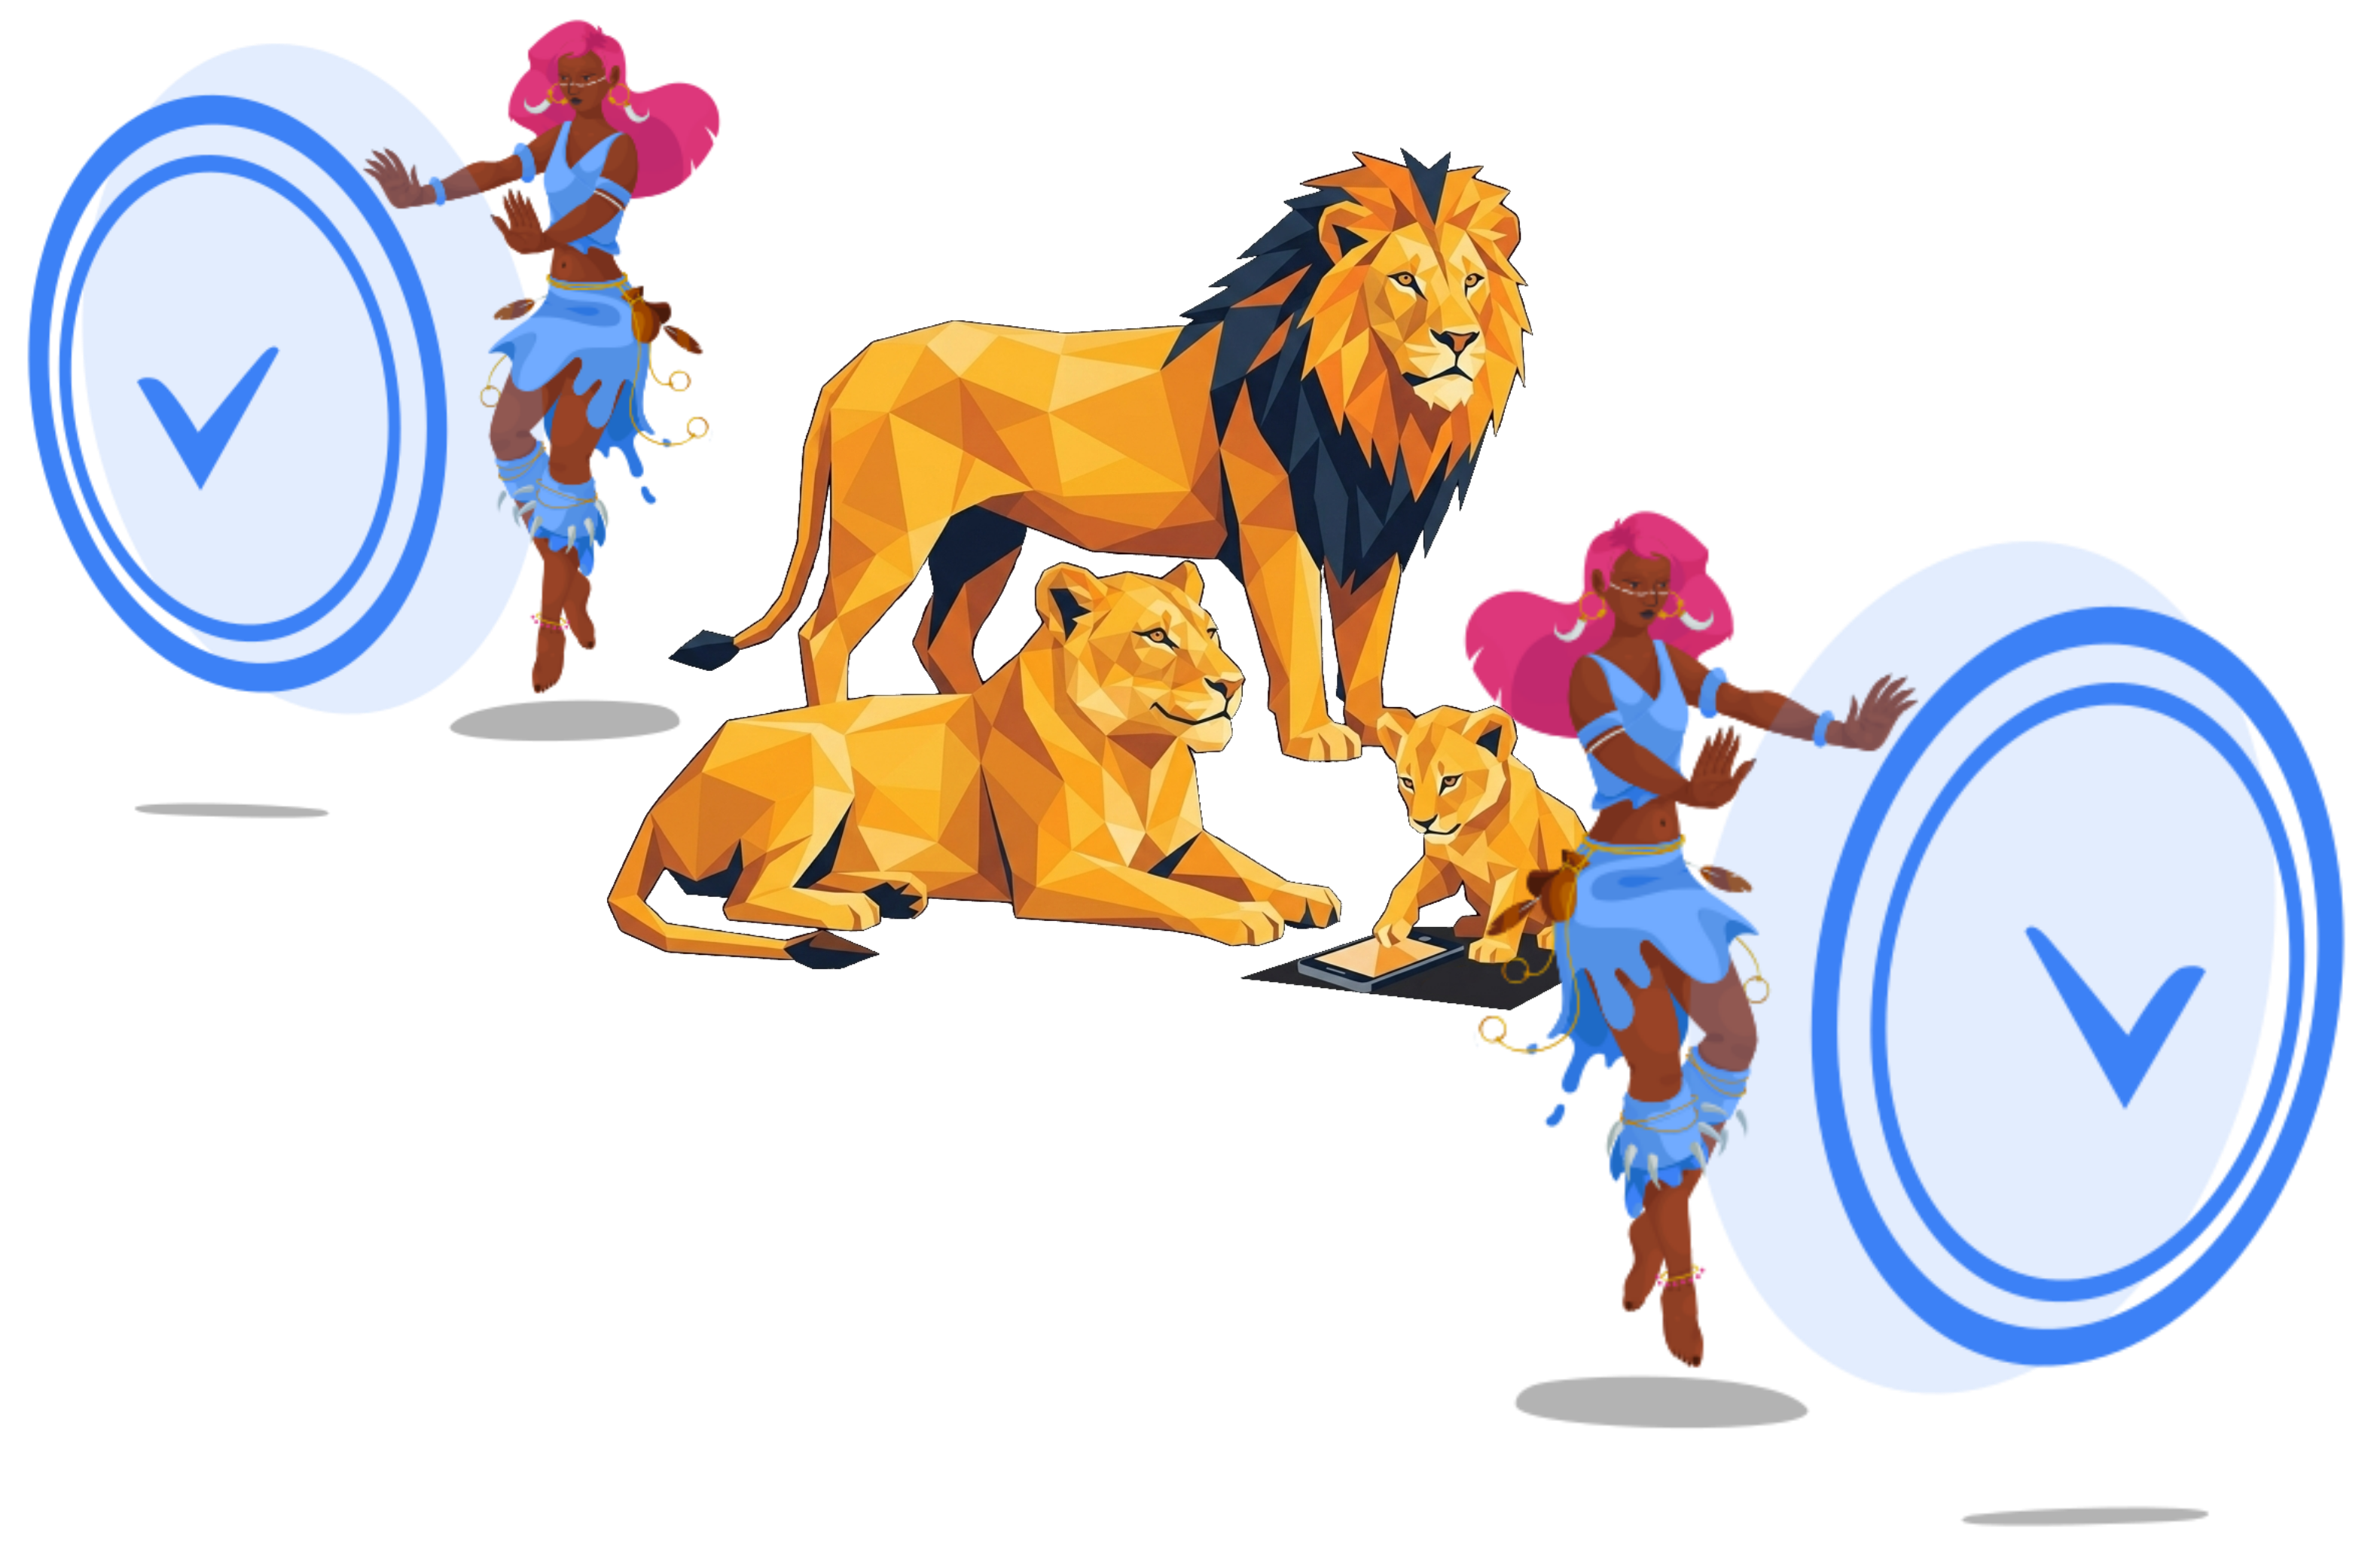
\includegraphics[width=0.8\textwidth]{imagens/capa_um.png} % Certifique-se que o nome bate
	\end{center}

	\vspace{1.5cm}
	
	% --- Informações do Projeto ---
	\vfill
	\textbf{Projeto de Atividade Extensionista I}\\
	Alinhado aos ODS 5 (Igualdade de Gênero) e 10 (Redução das Desigualdades)
	
	\vspace{1cm}
	
	\textbf{Autor:} Naygno Barbosa Noia\\
	\textit{CMEI Araras --- Palmas/TO}\\
	\textbf{Março de 2026}
\end{center}
	\newpage
	
	% 2. SUMÁRIO
	\tableofcontents 
	\newpage
	
	% 3. CORPO DO E-BOOK (Capítulos)
	\section*{Prefácio}

Se você está lendo este guia, parabéns: você decidiu assumir o controle da sua vida digital. 


Durante o nosso encontro no CMEI Araras, no dia 16 de março de 2026, compartilhamos histórias, medos e descobertas sobre como a tecnologia impacta o nosso dia a dia. Percebemos que a internet não precisa ser um lugar assustador e que não é necessário ser um gênio da informática para se proteger.


Muitas vezes, a tecnologia é desenhada para ser complexa, o que acaba afastando as pessoas e criando vulnerabilidades, principalmente em questões financeiras e na proteção das nossas crianças. A missão deste guia é quebrar essa barreira.


Assim como trancamos a porta de casa e olhamos para os dois lados antes de atravessar a rua, no mundo digital nós só precisamos criar novos (e simples) hábitos para navegar com paz interior.


Use este guia como o seu manual de sobrevivência. Configure seu celular no seu tempo, sem pressa. E, acima de tudo, compartilhe este conhecimento com suas amigas, alunos e familiares. A verdadeira segurança digital acontece quando cuidamos uns dos outros.


Uma excelente leitura e uma navegação segura!


\vspace{0.5cm}
\textbf{Naygno Barbosa Noia} \\
\textit{Ciência da Computação - UFBRA}

\vspace{1cm}
\begin{tcolorbox}[colback=NordBackground, colframe=BraveOrange, title=\faGithub\ Código Aberto (Open Source)]
	\textcolor{white}{Este guia foi totalmente tipografado em \LaTeX\ e seu código-fonte é aberto. Sinta-se à vontade para acessar o repositório no GitHub para sugerir melhorias ou compartilhar:}
	
	\vspace{0.3cm}
	\centering
	\href{https://github.com/naygno/guia-seguranca-cmei-araras}{\textbf{\textcolor{BitwardenBlue}{\faLink\ github.com/naygno/guia-seguranca-cmei-araras}}}
\end{tcolorbox}
	\newpage
	\section{Limpando a Poluição na Web: O Navegador Brave \faShield*}

A Web que usamos hoje não é gratuita; nós pagamos por ela com os nossos dados. Navegadores tradicionais (como Chrome ou Edge) foram projetados para rastrear o que você pesquisa, quanto tempo você olha para uma imagem e o que você pretende comprar. 

\vspace{0.3cm}
\noindent
Como vimos em nossa oficina, o problema não são apenas os \enquote{biscoitos} (cookies) que você aceita. Hoje, as empresas usam técnicas avançadas chamadas de \textit{Fingerprinting} (Impressão Digital do Dispositivo). Elas olham o tamanho da sua tela, a marca do seu celular e a sua bateria para saber quem você é, mesmo no \enquote{Modo Anônimo}.

\vspace{0.3cm}
\noindent
A solução para isso não é parar de navegar pela Web, mas sim usar um \textbf{Escudo Ativo}: o navegador \textbf{Brave}.

\vspace{0.3cm} % Respiro
\begin{figure}[h]
	\centering
	
\includegraphics[width=0.6\textwidth]{imagens/brave_color_darkbackground.png}
	\caption*{(\citeauthor{brave_app} \citefield{brave_app}{version} - Versão oficial)}
\end{figure}

\subsection*{Por que usar o Brave no dia a dia?}

\begin{itemize}
	\item \textbf{Bloqueio Nativo de Anúncios:} Ele remove propagandas chatas de sites e vídeos do YouTube automaticamente.
	\item \textbf{Navegação Web mais Rápida:} Como o celular não precisa baixar os \enquote{espiões} e os banners de propaganda, os sites carregam até 3x mais rápido, economizando a sua franquia de dados 4G.
	\item \textbf{Não requer ser um gênio da informática:} Você não precisa instalar extensões difíceis. É só baixar e usar. O Brave bloqueia as invasões \enquote{de fábrica}.
\end{itemize}

\subsection*{Passo a Passo para Limpar sua Navegação:}

\begin{enumerate}
	\item Abra a loja de aplicativos do seu celular (Play Store ou App Store) e pesquise por \textbf{Brave Browser}. Para facilitar, você pode simplesmente \textbf{tocar nas imagens abaixo} (se estiver lendo no celular) ou \textbf{escanear o QR Code} com a câmera para ser levado direto ao aplicativo oficial.
	
	\vspace{0.3cm} % Respiro
	\begin{center}
		\begin{minipage}{\linewidth}
			
			\begin{minipage}{0.3\linewidth}
				\centering
				\textbf{\textcolor{BraveOrange}{\faAndroid \ Android}}\\[0.2cm]
				\href{https://bfaxke.short.gy/brave-browser-android}{
					
\includegraphics[width=0.8\linewidth]{imagens/qr_brave_android.png}
				}\\[0.1cm]
				{\scriptsize (Toque ou escaneie)}
			\end{minipage}
			\hfill
			\begin{minipage}{0.3\linewidth}
				\centering
				\textbf{\textcolor{NordText}{\faApple \ iOS / iPhone}}\\[0.2cm]
				\href{https://bfaxke.short.gy/brave-browser-ios}{
					
\includegraphics[width=0.8\linewidth]{imagens/qr_brave_ios.png}
				}\\[0.1cm]
				{\scriptsize (Toque ou escaneie)}
			\end{minipage}
			\hfill
			\begin{minipage}{0.3\linewidth}
				\centering
				\textbf{\textcolor{BitwardenBlue}{\faDesktop \ Computador}}\\[0.2cm]
				\href{https://bfaxke.short.gy/brave-desktop}{
					
\includegraphics[width=0.8\linewidth]{imagens/qr_brave_desktop.png}
				}\\[0.1cm]
				{\scriptsize (Para Windows/Linux/Mac)}
			\end{minipage}
			
		\end{minipage}
	\end{center}
	\vspace{0.3cm} % Respiro após as imagens
	
	\item Instale o aplicativo \textbf{Brave} (o do Leão Laranja). 
	\item Ao abrir pela primeira vez, ele perguntará se deseja torná-lo seu \enquote{Navegador Padrão}. Escolha \textbf{Sim} (ou \enquote{Definir como padrão}). Isso garante que, ao clicar em um link no WhatsApp, você já abra protegido.
	\item \textbf{Pronto!} Agora, sempre que for pesquisar algo, ler notícias ou abrir o YouTube, use o Brave. 
\end{enumerate}

\subsubsection*{Ocultando Elementos Irritantes da Tela}

Assim como a privacidade do Brave, a função de \enquote{Bloqueio de Elementos} já vem nativamente integrada ao navegador. Você não precisa instalar extensões de terceiros, que frequentemente deixam o celular lento \cite{Brave2026}. Essa ferramenta permite esconder banners, janelas de aviso ou imagens chatas que atrapalham a sua leitura. Vejamos como usá-la no Android.

\vspace{0.3cm}
\noindent
Acesse uma página de sua preferência --- neste exemplo, utilizamos o portal de \textit{Minijogos} \cite{Minijogos2026}. Imediatamente ao abrir um site invasivo como este, o Brave inicia o bloqueio proativo de \textit{scripts}. É crucial entender que a grande maioria desses arquivos invisíveis atua como rastreadores silenciosos (\textit{trackers}), coletando dados sobre o seu hábito de navegação \cite{NIST2017}.

\vspace{0.3cm}
\noindent
Para ocultar algo que o Brave não escondeu sozinho, siga as etapas:
\vspace{0.3cm}

% --- BLOCO DE IMAGENS 1 ---
\noindent
\begin{minipage}{\textwidth}
	\centering
	\begin{minipage}{0.45\textwidth}
		\centering
		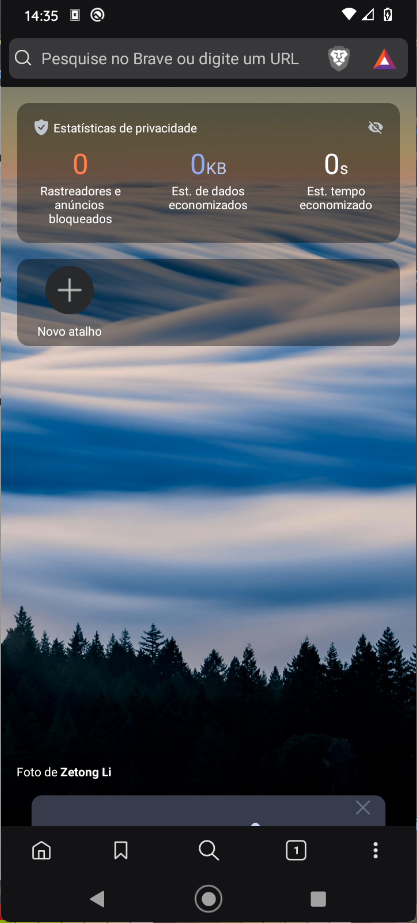
\includegraphics[trim={0cm 15cm 0cm 0cm}, clip, width=\textwidth]{imagens/brave_bloqueio_elementos_01.png}\\[0.2cm]
		\passo{BraveOrange}{1}{Entre em um site}
	\end{minipage}
	\hfill
	\begin{minipage}{0.45\textwidth}
		\centering
		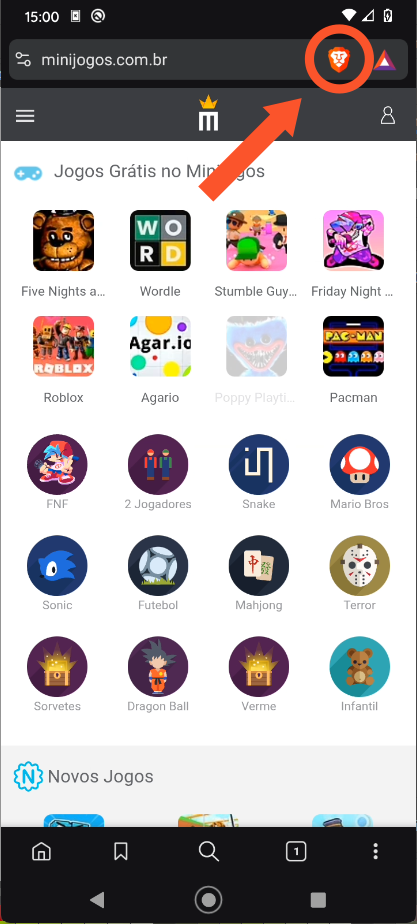
\includegraphics[trim={0cm 15cm 0cm 0cm}, clip, width=\textwidth]{imagens/brave_bloqueio_elementos_02.png}\\[0.2cm]
		\passo{BraveOrange}{2}{Toque no Leãozinho}
	\end{minipage}
\end{minipage}

\vspace{0.3cm}
\noindent
Ao efetuar o Passo 2, o painel de proteção (Escudos) se abrirá.

\vspace{0.3cm}
% --- BLOCO DE IMAGENS 2 ---
\noindent
\begin{minipage}{\textwidth}
	\centering
	\begin{minipage}{0.45\textwidth}
		\centering
		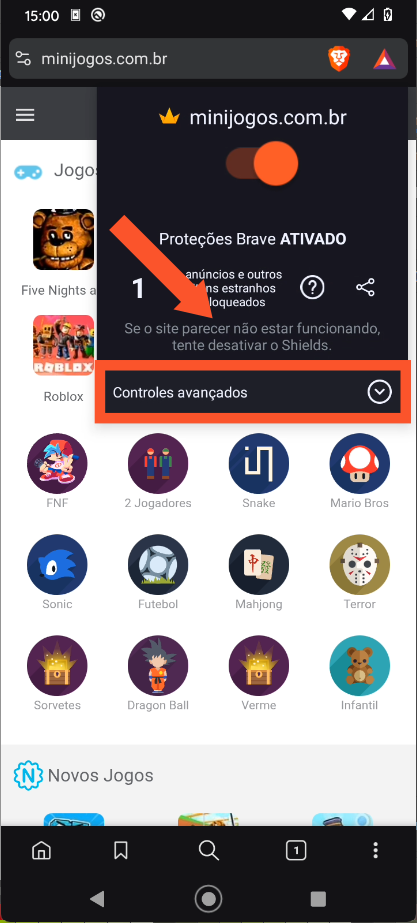
\includegraphics[trim={0cm 0cm 0cm 0cm}, clip, width=\textwidth]{imagens/brave_bloqueio_elementos_03.png}\\[0.2cm]
		\passo{BraveOrange}{3}{Toque em \enquote{Controles Avançados}}
	\end{minipage}
	\hfill
	\begin{minipage}{0.45\textwidth}
		\centering
		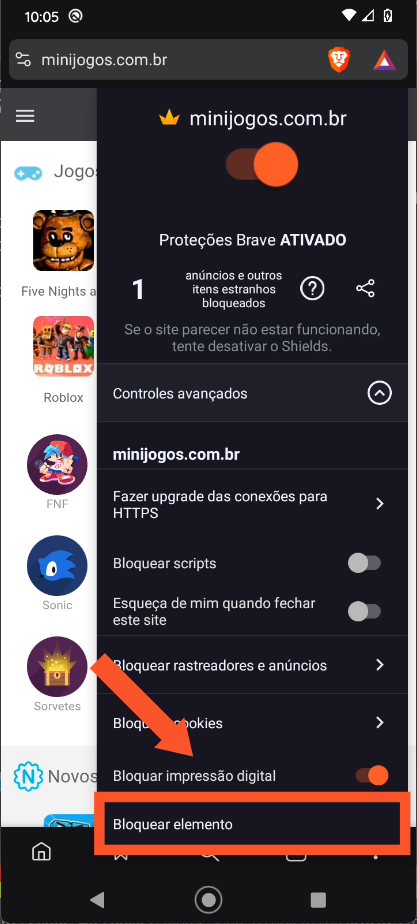
\includegraphics[trim={0cm 0cm 0cm 0cm}, clip, width=\textwidth]{imagens/brave_bloqueio_elementos_04.png}\\[0.2cm]
		\passo{BraveOrange}{4}{Toque em \enquote{Bloquear elemento}}
	\end{minipage}
\end{minipage}

\vspace{0.5cm}

% --- BLOCO DE IMAGENS 3 ---
\noindent
\begin{minipage}{\textwidth}
	\centering
	\begin{minipage}{0.45\textwidth}
		\centering
		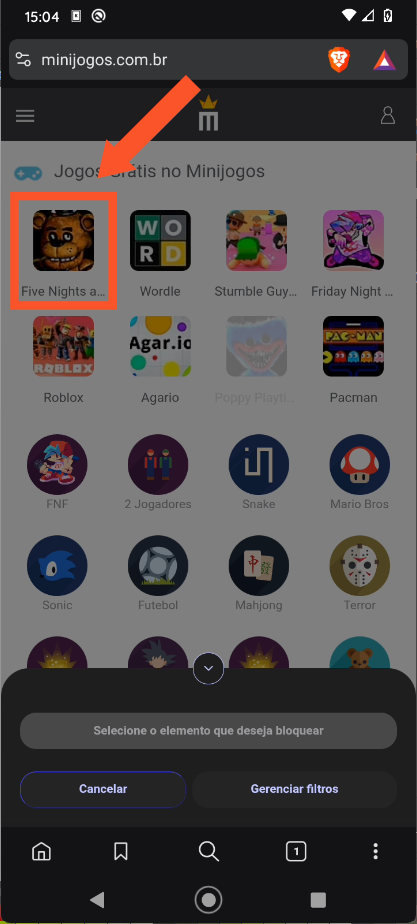
\includegraphics[trim={0cm 0cm 0cm 0cm}, clip, width=\textwidth]{imagens/brave_bloqueio_elementos_05.png}\\[0.2cm]
		\passo{BraveOrange}{5}{Selecione o item \enquote{indesejado}}
	\end{minipage}
	\hfill
	\begin{minipage}{0.45\textwidth}
		\centering
		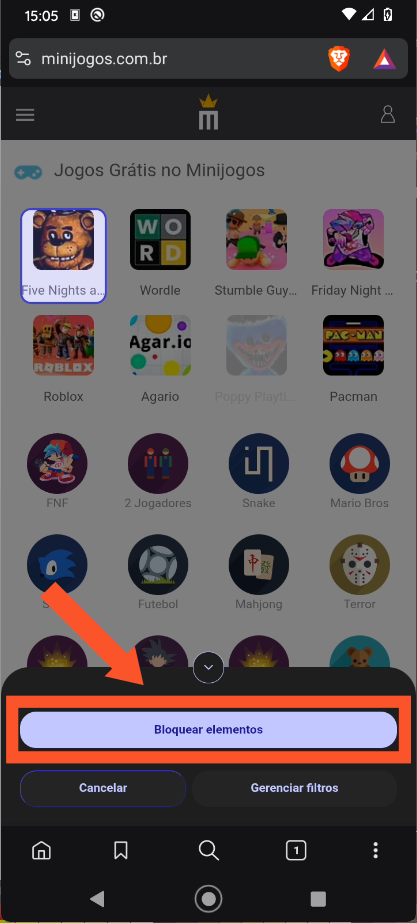
\includegraphics[trim={0cm 0cm 0cm 0cm}, clip, width=\textwidth]{imagens/brave_bloqueio_elementos_06.png}\\[0.2cm]
		\passo{BraveOrange}{6}{Confirme no botão azul}
	\end{minipage}
\end{minipage}

\vspace{0.3cm}
\noindent
Parabéns! O elemento indesejado desapareceu da sua tela. Caso você se arrependa ou esconda o elemento errado sem querer, é muito fácil reverter a ação:

\vspace{0.3cm}
% --- BLOCO DE IMAGENS 4 ---
\noindent
\begin{minipage}{\textwidth}
	\centering
	\begin{minipage}{0.45\textwidth}
		\centering
		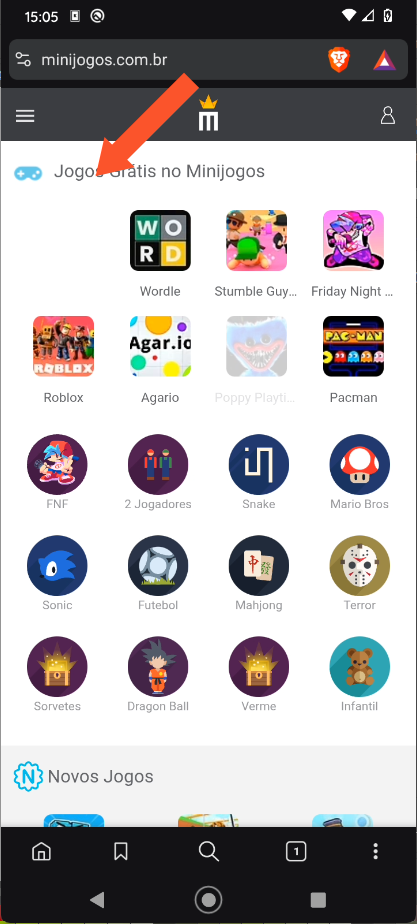
\includegraphics[trim={0cm 15cm 0cm 0cm}, clip, width=\textwidth]{imagens/brave_bloqueio_elementos_07.png}\\[0.2cm]
		\passo{BraveOrange}{7}{O item desapareceu da tela}
	\end{minipage}
	\hfill
	\begin{minipage}{0.45\textwidth}
		\centering
		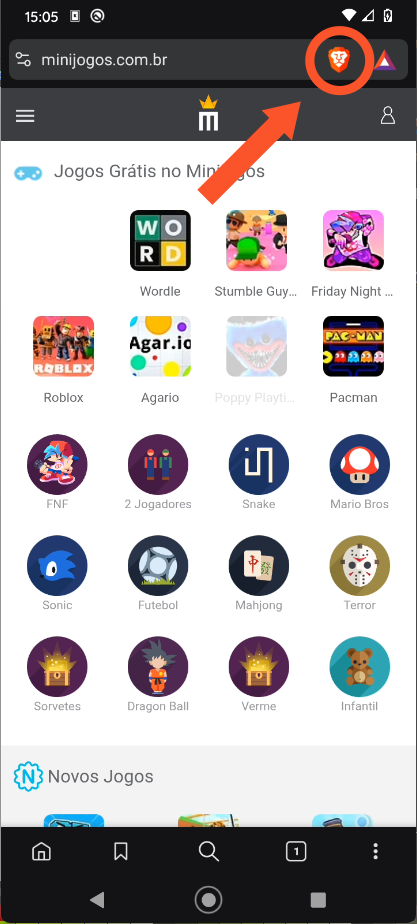
\includegraphics[trim={0cm 15cm 0cm 0cm}, clip, width=\textwidth]{imagens/brave_bloqueio_elementos_08.png}\\[0.2cm]
		\passo{BraveOrange}{8}{Abra o menu do Leãozinho novamente}
	\end{minipage}
\end{minipage}

\vspace{0.5cm}

% --- BLOCO DE IMAGENS 5 ---
\noindent
\begin{minipage}{\textwidth}
	\centering
	\begin{minipage}{0.45\textwidth}
		\centering
		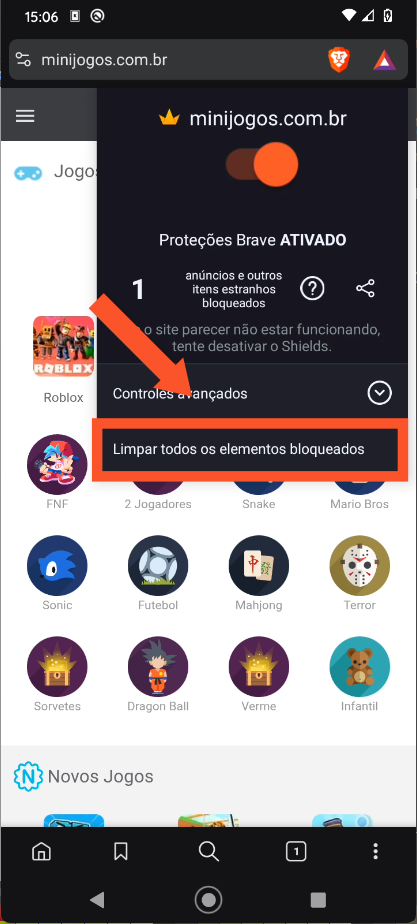
\includegraphics[trim={0cm 10cm 0cm 0cm}, clip, width=\textwidth]{imagens/brave_bloqueio_elementos_09.png}\\[0.2cm]
		\passo{BraveOrange}{9}{Toque em \enquote{Limpar elementos}}
	\end{minipage}
	\hfill
	\begin{minipage}{0.45\textwidth}
		\centering
		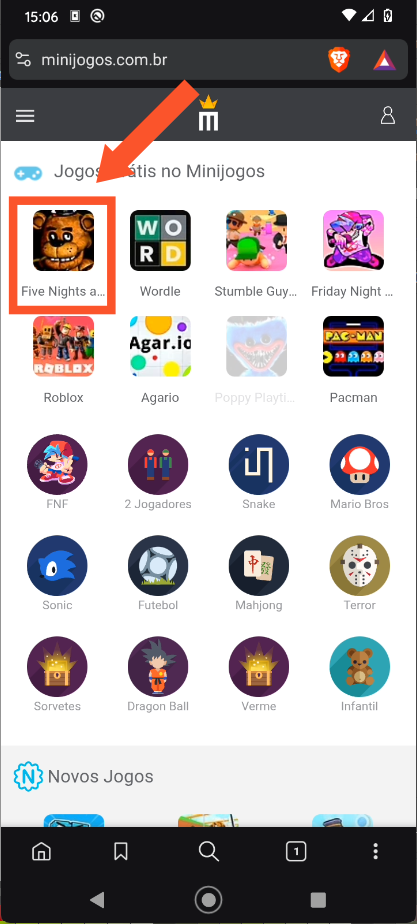
\includegraphics[trim={0cm 10cm 0cm 0cm}, clip, width=\textwidth]{imagens/brave_bloqueio_elementos_10.png}\\[0.2cm]
		\passo{BraveOrange}{10}{O item original retornou à página}
	\end{minipage}
\end{minipage}


\vspace{0.3cm}
\noindent
Explore os \enquote{Controles Avançados} no menu do Leãozinho Corajoso para personalizar ainda mais sua segurança:

\begin{itemize}
	\item \textbf{Fazer upgrade para HTTPS:} Esta opção força a conexão a ser criptografada (o famoso \enquote{Cadeado} na barra de endereço). É uma camada essencial para proteger suas senhas em redes públicas.
	\item \textbf{Bloquear rastreadores e anúncios:} Em sites muito poluídos, mude para \enquote{Agressivo}. O site ficará extremamente limpo e rápido.
	\item \textbf{Bloquear cookies:} Use com cautela. Se ativado para \enquote{Todos}, sites como o Facebook ou o portal da escola vão deslogar a sua conta a cada clique. Deixe na opção padrão de bloqueio de \enquote{Terceiros}.
	\item \textbf{Bloquear impressão digital:} Oculte o modelo do seu celular e a sua placa de vídeo dos sites. É o seu \enquote{Disfarce Digital}.
\end{itemize} 

\begin{tcolorbox}[colback=NordBackground, colframe=BraveOrange, coltext=white, % <--- Isso garante que TODO o texto dentro da caixa seja branco 
	title=\faYoutube \ \textbf{Dica de Ouro para as Mãe}s
	]
	Se você quiser deixar a criança assistindo a desenhos no celular sem o risco de aparecerem propagandas no meio do vídeo, basta abrir o site do YouTube diretamente \textbf{dentro} do navegador Brave. A mágica acontece na hora!
\end{tcolorbox}
	\newpage
	\section{O Mestre das Chaves: Cofre Bitwarden \faKey}

O nome do seu cachorro não é uma senha segura, e anotar senhas em um caderno é muito perigoso. O segredo da segurança não é a dificuldade (símbolos estranhos), é o \textbf{TAMANHO}. 

\vspace{0.3cm}
Tentar decorar senhas para 50 sites diferentes é impossível. É por isso que usamos um \textbf{Gerenciador de Senhas}.

\vspace{0.3cm}
\begin{figure}[h]
	\centering
	%\imagemSuave[0.6\textwidth]{imagens/cofre_bitwarden.png} 
	
\includegraphics[width=0.6\textwidth]{imagens/bitwarden_logo.png}
		\caption*{(\citeauthor{bitwarden_app} \citefield{bitwarden_app}{version} - Versão oficial)}
\end{figure}

\subsection*{Como criar o seu Cofre Digital:}
\begin{enumerate}
	\item Baixe o aplicativo \textbf{Bitwarden} no seu celular.

	\begin{center}
		\begin{minipage}{\linewidth}
			
			\begin{minipage}{0.3\linewidth}
				\centering
				\textbf{\textcolor{BraveOrange}{\faAndroid \ Android}}\\[0.2cm]
				\href{https://bfaxke.short.gy/bitwarden-android}{
					
\includegraphics[width=0.8\linewidth]{imagens/qr_bitwarden_android.png}
				}\\[0.1cm]
				{\scriptsize (Toque ou escaneie)}
			\end{minipage}
			\hfill
			\begin{minipage}{0.3\linewidth}
				\centering
				\textbf{\textcolor{NordText}{\faApple \ iOS / iPhone}}\\[0.2cm]
				\href{https://bfaxke.short.gy/bitwarden-apple}{
					
\includegraphics[width=0.8\linewidth]{imagens/qr_bitwarden_ios.png}
				}\\[0.1cm]
				{\scriptsize (Toque ou escaneie)}
			\end{minipage}
			\hfill
			\begin{minipage}{0.3\linewidth}
				\centering
				\textbf{\textcolor{BitwardenBlue}{\faDesktop \ Computador}}\\[0.2cm]
				\href{https://bfaxke.short.gy/bitwarden-desktop}{
					
\includegraphics[width=0.8\linewidth]{imagens/qr_bitwarden_desktop.png}
				}\\[0.1cm]
				{\scriptsize (Para Windows/Linux/Mac)}
			\end{minipage}
			
		\end{minipage}
	\end{center}
	
	\item Crie uma conta usando o seu e-mail.
	\item Invente UMA única \textbf{\enquote{Senha Mestra}}. Use uma frase longa que faça sentido para você (Exemplo: \textit{\enquote{Eu amo bolo de cenoura com cafe}}).
	\item Vá nas \textit{Configurações > Segurança} do aplicativo e ative o \textbf{Desbloqueio por Biometria} (Impressão Digital).
\end{enumerate}

\subsection*{Passo a Passo para Configurar o Bitwarden:}

\subsection*{Muito Além das Senhas: Sua Carteira Blindada}

O Bitwarden não guarda apenas senhas. Ele é um cofre digital completo desenhado para substituir a sua carteira física e a sua agenda de anotações. Ao clicar no botão de adicionar (\textbf{+}), você descobrirá diferentes \enquote{Tipos} de documentos que podem ser trancados com a sua biometria:

\begin{itemize}
	\item \textbf{Cartões de Crédito:} Guarde os dados dos seus cartões físicos e virtuais de forma criptografada. É infinitamente mais seguro do que deixar salvo no bloco de notas do celular ou tirar foto do cartão.
	\item \textbf{Identidades:} Salve seu CPF, RG, Passaporte e Endereço completo. Assim, quando for preencher um formulário longo em um site seguro, o Bitwarden preenche tudo para você.
	\item \textbf{Anotações Seguras:} Sabe a senha do Roteador Wi-Fi ou aquele \enquote{Código de Recuperação} do WhatsApp? Crie uma anotação segura para que só você tenha acesso.
\end{itemize}

\subsection*{A Configuração do PIN e a Pergunta Crítica}

Ao configurar o acesso rápido (Biometria ou PIN) para não ter que digitar sua frase-senha o tempo todo, o aplicativo fará uma pergunta muito importante: \textbf{\enquote{Exigir senha principal no reinício do aplicativo?}}

\begin{figure}[h]
	\centering
	% Substitua pelo nome do seu arquivo da Imagem 6
	\imagemSuave[0.6\linewidth]{imagens/bitwarden_aviso_reinicio.png}
\end{figure}

\begin{tcolorbox}[colback=NordBackground, colframe=BraveOrange, coltext=white, title=\faShieldAlt \ Qual a diferença entre Sim e Não?]
	\textbf{Se você escolher \enquote{NÃO}:} O aplicativo deixará uma cópia da sua chave do cofre no celular, protegida apenas pelo seu PIN. É prático, mas se o seu celular for roubado, um PIN de 4 números é fácil de ser quebrado por criminosos.
	
	\textbf{Se você escolher \enquote{SIM} (Nossa Recomendação):} O celular nunca guarda a chave. Se o aparelho for roubado e desligado, o cofre se tranca totalmente. Quando o celular for reiniciado, você terá que digitar a sua \enquote{Senha Mestra} (a frase longa) uma vez para reabrir o cofre. No dia a dia normal, o seu PIN e a sua digital continuarão funcionando rapidamente!
\end{tcolorbox}

\begin{tcolorbox}[colback=NordBackground, colframe=BraveOrange, title=\faExclamationTriangle\ A Regra de Ouro]
	\textcolor{white}{O Bitwarden não possui a opção \enquote{Esqueci minha senha}. Anote a sua Senha Mestra em um pedaço de papel e guarde no fundo de uma gaveta segura na sua casa. Se esquecer a senha mestra, o cofre ficará trancado para sempre!}
\end{tcolorbox}
	\newpage
	\section{Protegendo as Crianças: O Filtro AdGuard \faChild}

Como garantir que seu filho não acesse sites adultos, de violência extrema ou de apostas no celular? Nós vamos colocar um filtro direto no \enquote{cano} de internet do aparelho.

Diferente de aplicativos espiões pesados, essa é uma configuração \enquote{escondida} no próprio sistema do seu celular que limpa a internet antes mesmo de ela aparecer na tela.

\subsection*{Como configurar no Android:}
\begin{enumerate}
	\item Abra as \textbf{Configurações} do celular.
	\item Procure por \textbf{Rede e Internet} (ou use a Lupa \faSearch\ e digite ``DNS'').
	\item Clique na opção \textbf{DNS Privado}.
	\item Marque a opção \textit{\enquote{Nome do host do provedor de DNS}}.
	\item Digite exatamente este código (tudo minúsculo): 
	
	\begin{center}
		\textbf{\textcolor{AdguardGreen}{family.adguard-dns.com}}
	\end{center}
	
	\item Clique em \textbf{Salvar}.
\end{enumerate}

\begin{tcolorbox}[colback=NordBackground, colframe=AdguardGreen, title=\faCheckCircle\ Vantagem Extra]
	\textcolor{white}{Além de proteger as crianças contra sites perigosos, este filtro também bloqueia boa parte das propagandas em jogos e aplicativos gratuitos!}
\end{tcolorbox}
	\newpage
	\section{Protegendo seu Bolso e sua Mente \faCreditCard}

A tecnologia avança, mas o alvo do criminoso continua sendo o seu dinheiro. Aqui estão as duas defesas finais para a sua rotina:

\subsection*{1. O Cartão Bancário que Desaparece (Cartão Virtual)}
Nunca digite o número do seu cartão de plástico na internet. No aplicativo do seu banco, gere um \textbf{Cartão Virtual}. 
Ele funciona como uma nota de dinheiro mágica: você paga e o número deixa de existir. Se o site for falso e invadido, o hacker roubará um número inútil, e o seu cartão físico na sua carteira continuará seguro.

\subsection*{2. O Golpe da Maquininha no Ônibus}
Para evitar que criminosos encostem máquinas de cartão na sua bolsa no transporte público: entre no aplicativo do seu banco e \textbf{DESATIVE} a opção de \textit{\enquote{Pagamento por aproximação (NFC)}} do seu cartão físico. Se for pagar por aproximação, prefira usar o celular.

\vspace{0.5cm}

\begin{tcolorbox}[colback=NordBackground, colframe=red, title=\faBrain\ \textbf{A Regra de Ouro: Engenharia Social}]
	\textcolor{white}{\textbf{O bandido não hackeia o seu celular, ele hackeia a sua mente.}}\\
	\textcolor{white}{Se uma mensagem no WhatsApp causar \textbf{URGÊNCIA} (\enquote{sua conta será bloqueada em 30 min!}) ou \textbf{MEDO} (\enquote{mãe, perdi meu celular, manda um pix.}), \textbf{PARE E RESPIRE}. A pressa é a principal arma deles. Nunca clique em links. Feche a mensagem e ligue para a pessoa para ouvir a voz dela.}
\end{tcolorbox}
	\newpage
	\section{A Máscara: Privacidade de E-mail \faUserSecret}

Seu e-mail principal (aquele que você usa no banco e no celular) é como a \textbf{chave da sua casa}. Você não entrega a chave da sua casa para o caixa da farmácia só porque ele pediu para fazer um cadastro de desconto, certo? 

\vspace{0.3cm}
\noindent
Mas é exatamente isso que fazemos na internet. Toda vez que um site de compras, um Wi-Fi de shopping ou um aplicativo desconhecido pede o seu e-mail, você está entregando a sua chave principal. Se esse site for invadido por hackers, o seu e-mail verdadeiro cai nas mãos de criminosos, e a sua caixa de entrada lota de propagandas (SPAM) e tentativas de golpes.

\vspace{0.3cm}
\noindent
A solução para isso é usar uma \textbf{Máscara de E-mail}.

\subsection*{Como funciona a Máscara (O \enquote{Patinho} Protetor)}

Imagine que a Máscara de E-mail é uma \textbf{Caixa Postal Automática}. 
Em vez de dar o seu endereço real para a loja, você dá o e-mail da Caixa Postal. A loja manda a propaganda para lá. 

\vspace{0.3cm}
\noindent
O sistema do DuckDuckGo funciona como um \textbf{Scanner de Raio-X de aeroporto}: a máquina escaneia a mensagem, destrói os rastreadores invisíveis automaticamente e encaminha a mensagem limpa para o seu e-mail verdadeiro. 

\vspace{0.3cm} % Respiro
\begin{figure}[h]
	\centering
	
\includegraphics[width=0.7\textwidth]{imagens/duckduckgo_logo.png}
	\caption*{(\citeauthor{duckduckgo_app} \citefield{duckduckgo_app}{version} - Versão oficial)}
\end{figure}

\vspace{0.3cm}
\noindent
\textbf{A grande vantagem:} Se a loja começar a mandar lixo demais ou vazar seus dados, você simplesmente \enquote{explode} aquela Caixa Postal com um clique. O spam para na hora, e o seu e-mail verdadeiro continua secreto e seguro!

\vspace{0.3cm}

\begin{tcolorbox}[colback=NordBackground, colframe=DuckDuckGoOrange, coltext=white, title=\faShield* \ \textbf{Eles vão ler os meus e-mails?}]
	\textbf{NÃO.} O DuckDuckGo garante contratualmente que não lê nem armazena o conteúdo das suas mensagens. A remoção dos rastreadores é feita por computadores usando \textbf{Processamento em Memória (RAM)}. 
	
	\vspace{0.3cm}
	\noindent
	Isso significa que a mensagem é limpa e encaminhada em milissegundos, sem nunca ser gravada em um disco rígido. É um processo \enquote{cego} e criptografado, que respeita os mais altos padrões internacionais de privacidade e a nossa Lei Geral de Proteção de Dados (LGPD).
\end{tcolorbox}

\subsection*{\faLock \ Por que confiar no DuckDuckGo? \cite{DuckDuckGoPrivacy2023}}

Diferente de um serviço de e-mail comum, o \enquote{Patinho} não é um lugar onde você entra para ler mensagens. Ele é um \textbf{servidor de encaminhamento}.

\begin{itemize}
	\item \textbf{Não é uma nova conta:} Você não terá uma caixa de entrada no DuckDuckGo. Ele apenas \enquote{peneira} o que chega e joga para o seu e-mail pessoal.
	\item \textbf{Endereço Pessoal vs. Máscaras:} Ao se cadastrar, você cria o seu:
	\vspace{0.3cm}
	% Caixa isolada para facilitar a cópia no celular
	\noindent
	\begin{center}
		\begin{tcolorbox}[
			colback=NordBackground, 
			colframe=DuckDuckGoOrange, 
			width=0.8\linewidth, 
			halign=center,       % Centraliza horizontalmente
			valign=center,       % Centraliza verticalmente
			boxrule=1pt, 
			arc=2mm,
			top=3mm,             % Ajuste fino da margem superior
			bottom=3mm           % Ajuste fino da margem inferior
			]
			\Large \sffamily \textbf{\textcolor{DuckDuckGoOrange}{\textbf{seu-nome@duck.com}}}
		\end{tcolorbox}
	\end{center}
	\vspace{0.3cm}
	\textbf{Cuidado:} Não use esse endereço em sites duvidosos! Ele serve apenas como sua identificação no serviço. Para cadastros e compras, use sempre os \textbf{Endereços Privados} (gerados aleatoriamente).
	\item \textbf{Eles não guardam nada:} Suas mensagens passam pelo sistema como água por um cano. Nada fica gravado em discos rígidos.
	\item \textbf{Processamento cego:} A limpeza é feita na memória temporária (RAM). Nenhum ser humano ou robô lê o conteúdo do que você escreve.
\end{itemize}

\vspace{0.3cm}
\begin{center}
	\begin{minipage}{\linewidth}
		
		\begin{minipage}{0.3\linewidth}
			\centering
			\textbf{\textcolor{BraveOrange}{\faAndroid \ Android}}\\[0.2cm]
			\href{https://bfaxke.short.gy/duckduckgo-android}{
				
\includegraphics[width=0.8\linewidth]{imagens/qr_duckduckgo_android.png}
			}\\[0.1cm]
			{\scriptsize (Toque ou escaneie)}
		\end{minipage}
		\hfill
		\begin{minipage}{0.3\linewidth}
			\centering
			\textbf{\textcolor{NordText}{\faApple \ iOS / iPhone}}\\[0.2cm]
			\href{https://bfaxke.short.gy/duckduckgo-ios}{
				
\includegraphics[width=0.8\linewidth]{imagens/qr_duckduckgo_ios.png}
			}\\[0.1cm]
			{\scriptsize (Toque ou escaneie)}
		\end{minipage}
		\hfill
		\begin{minipage}{0.3\linewidth}
			\centering
			\textbf{\textcolor{BitwardenBlue}{\faDesktop \ Computador}}\\[0.2cm]
			\href{https://bfaxke.short.gy/duckduckgo-desktop}{
				
\includegraphics[width=0.8\linewidth]{imagens/qr_duckduckgo_desktop.png}
			}\\[0.1cm]
			{\scriptsize (Para Windows/Linux/Mac)}
		\end{minipage}
		
	\end{minipage}
\end{center}

\subsection*{Passo a Passo: Criando sua Primeira Máscara}

Para ativar essa proteção gratuita, você precisa do aplicativo do \textbf{DuckDuckGo} no celular/computar (ou da extensão no navegador). Vamos ver como ativar no celular. Após instalar, abra o DuckduckGo na página inicial como mostrado no \textbf{Passo 1} abaixo:

\vspace{0.5cm}

% --- BLOCO DE IMAGENS 1 ---
\noindent
\begin{minipage}{\textwidth}
	\centering
	\begin{minipage}{0.45\textwidth}
		\centering
		% Insira o print da tela inicial do App DuckDuckGo
		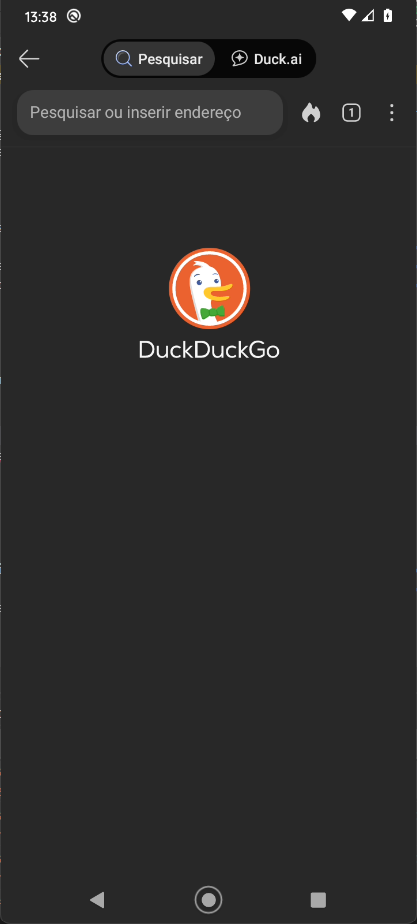
\includegraphics[trim={0cm 0cm 0cm 0cm}, clip, width=\textwidth]{imagens/duckduckgo_01.png}\\[0.2cm]
		\passo{DuckDuckGoOrange}{1}{Página inicial do DuckDuckGo}
	\end{minipage}
	\hfill
	\begin{minipage}{0.45\textwidth}
		\centering
		% Insira o print da opção Email Protection
		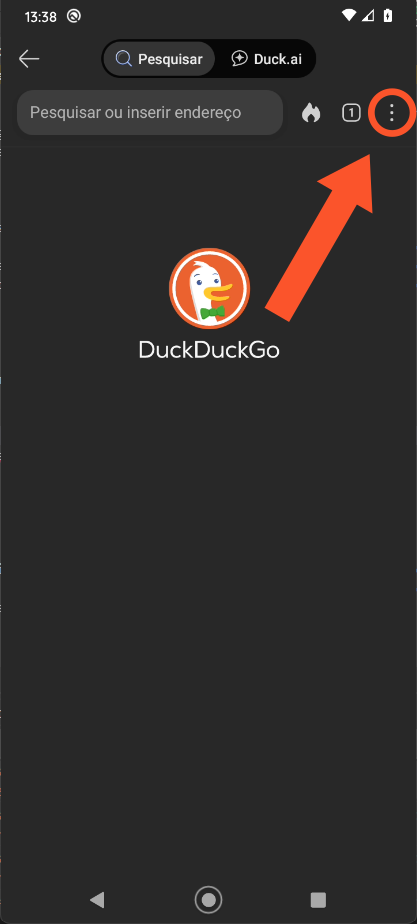
\includegraphics[trim={0cm 0cm 0cm 0cm}, clip, width=\textwidth]{imagens/duckduckgo_02.png}\\[0.2cm]
		\passo{DuckDuckGoOrange}{2}{Toque nos três pontinhos acima}
	\end{minipage}
\end{minipage}

\vspace{0.5cm}
\noindent
Feito a ação do \textbf{Passo 2} anterior, localize as \textbf{Definições} e toque nela como abaixo:

% --- BLOCO DE IMAGENS 2 ---
\noindent
\begin{minipage}{\textwidth}
	\centering
	\begin{minipage}{0.45\textwidth}
		\centering
		% Insira o print da tela de criar o endereço @duck.com
		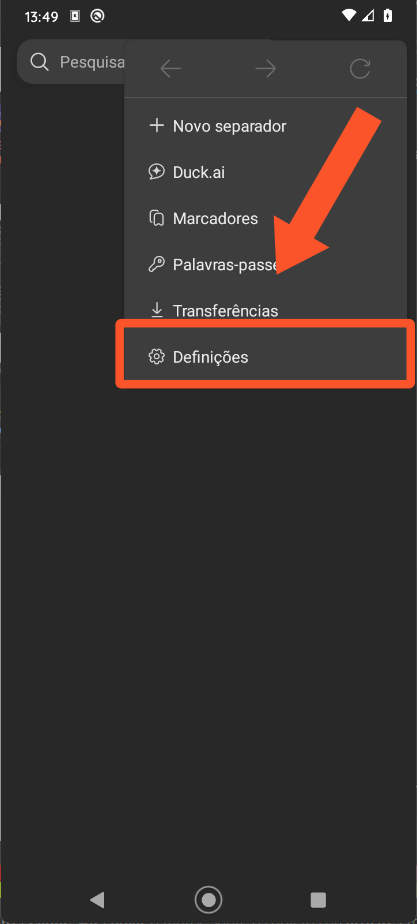
\includegraphics[trim={0cm 0cm 0cm 0cm}, clip, width=\textwidth]{imagens/duckduckgo_03.png}\\[0.2cm]
		\passo{DuckDuckGoOrange}{3}{Toque em \enquote{Definições}}
	\end{minipage}
	\hfill
	\begin{minipage}{0.45\textwidth}
		\centering
		% Insira o print de onde colocar o e-mail verdadeiro
		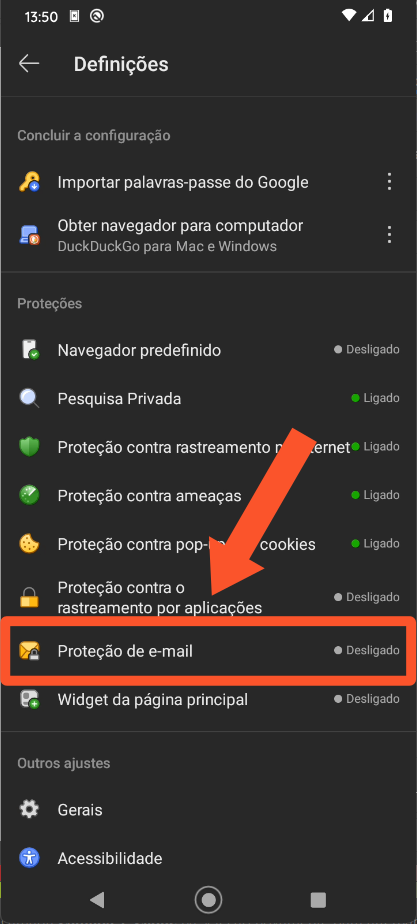
\includegraphics[trim={0cm 0cm 0cm 0cm}, clip, width=\textwidth]{imagens/duckduckgo_04.png}\\[0.2cm]
		\passo{DuckDuckGoOrange}{4}{Vá em \enquote{Proteção de e-mail}}
	\end{minipage}
\end{minipage}

\vspace{0.5cm}
\noindent
No \textbf{Passo 4} acima, note que a opção \enquote{Proteção de e-mail} está definida com \textbf{Desligado}. Então precisamos ligá-la, vamos fazer isso nos próximos passos.

% --- BLOCO DE IMAGENS 3 ---
\noindent
\begin{minipage}{\textwidth}
	\centering
	\begin{minipage}{0.45\textwidth}
		\centering
		% Insira o print da tela de criar o endereço @duck.com
		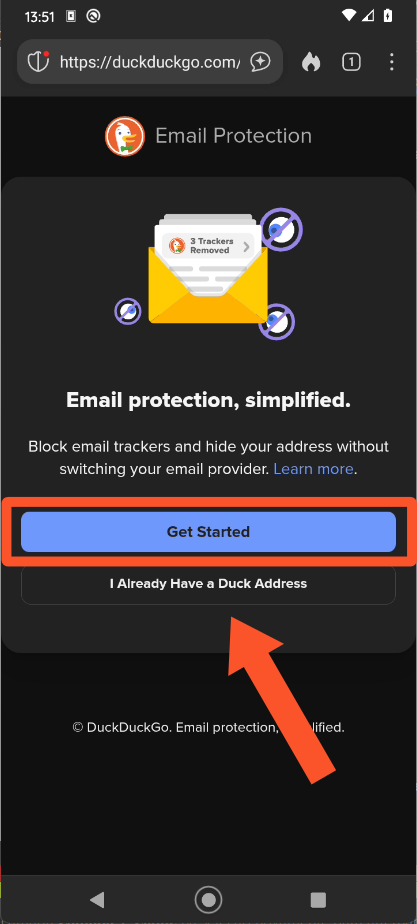
\includegraphics[trim={0cm 0cm 0cm 0cm}, clip, width=\textwidth]{imagens/duckduckgo_05.png}\\[0.2cm]
		\passo{DuckDuckGoOrange}{5}{Toque em \enquote{Get Started} (Comece)}
	\end{minipage}
	\hfill
	\begin{minipage}{0.45\textwidth}
		\centering
		% Insira o print de onde colocar o e-mail verdadeiro
		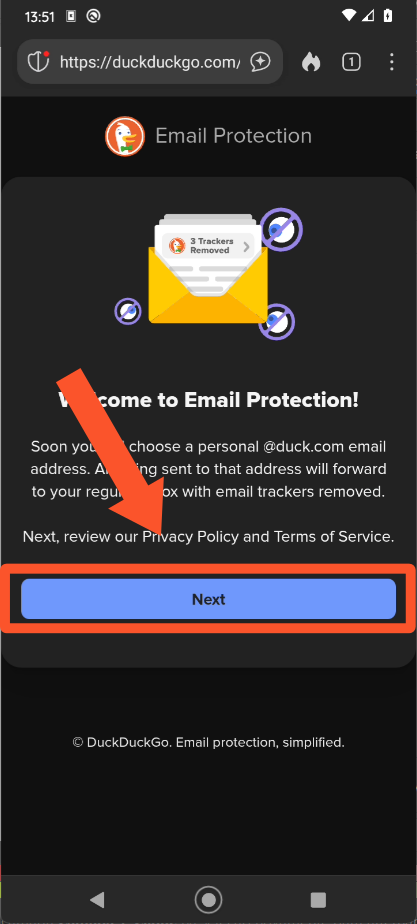
\includegraphics[trim={0cm 0cm 0cm 0cm}, clip, width=\textwidth]{imagens/duckduckgo_06.png}\\[0.2cm]
		\passo{DuckDuckGoOrange}{6}{Toque em \enquote{Next} (Próximo)} \newline
	\end{minipage}
\end{minipage}

\vspace{0.3cm}
\noindent

% --- BLOCO DE IMAGENS 4 ---
\noindent
\begin{minipage}{\textwidth}
	\centering
	\begin{minipage}{0.45\textwidth}
		\centering
		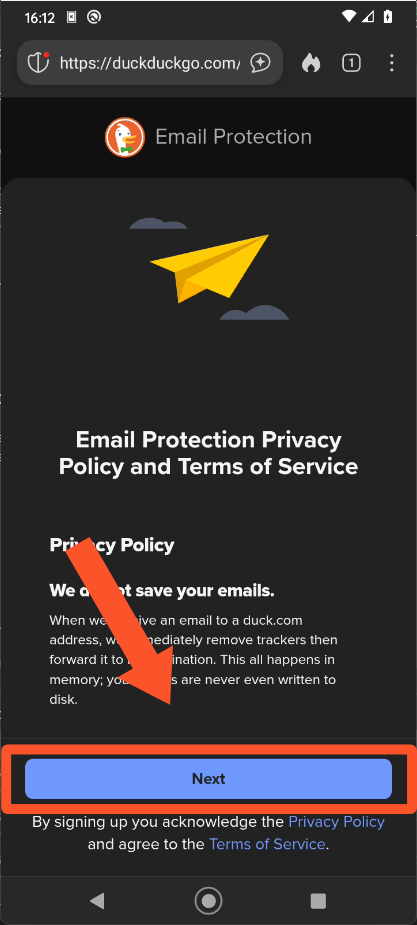
\includegraphics[trim={0cm 0cm 0cm 0cm}, clip, width=\textwidth]{imagens/duckduckgo_07.png}\\[0.2cm]
		\passo{BraveOrange}{7}{Toque no botão azul \enquote{Continue}}
	\end{minipage}
	\hfill
	\begin{minipage}{0.45\textwidth}
		\centering
		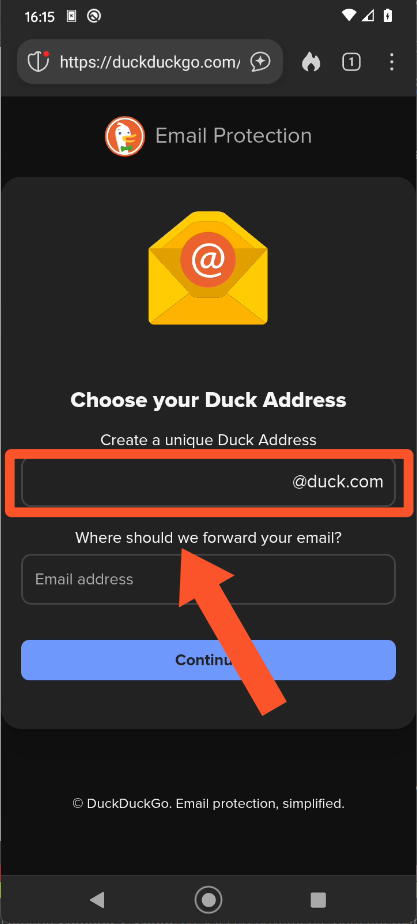
\includegraphics[trim={0cm 0cm 0cm 0cm}, clip, width=\textwidth]{imagens/duckduckgo_08.png}\\[0.2cm]
		\passo{BraveOrange}{8}{Escolha apenas o seu \enquote{Nome de Usuário}}
	\end{minipage}
\end{minipage}

\vspace{0.5cm}

\begin{tcolorbox}[colback=NordBackground, colframe=red, coltext=white, title=\faExclamationTriangle \ \textbf{Cuidado neste passo!}]
	\justifying \noindent
	No \textbf{Passo 8}, você deve digitar \textbf{APENAS} um nome (como se fosse um apelido):
	\begin{itemize}[label={}]
		\item \textbf{\textcolor{red}{\faTimesCircle \ ERRADO:}} \textbf{fulanodetal@gmail.com}
		\item \textbf{\textcolor{green}{\faCheckCircle \ CORRETO:}} \textbf{fulanodetal}
	\end{itemize}
	\noindent O final \textbf{@duck.com} já é colocado automaticamente pelo sistema. Não use espaços ou símbolos especiais.
\end{tcolorbox}

\vspace{0.3cm}
\noindent

% --- BLOCO DE IMAGENS 5 ---
\noindent
\begin{minipage}{\textwidth}
	\centering
	\begin{minipage}{0.45\textwidth}
		\centering
		% Insira o print da tela de criar o endereço @duck.com
		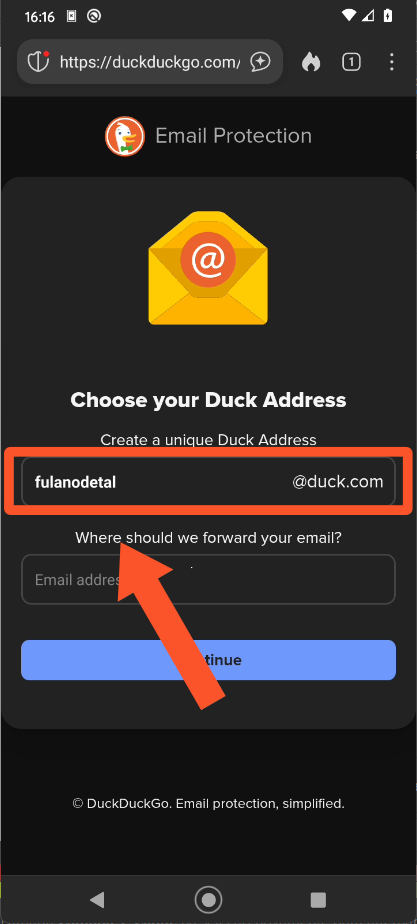
\includegraphics[trim={0cm 0cm 0cm 0cm}, clip, width=\textwidth]{imagens/duckduckgo_09.png}\\[0.2cm]
		\passo{DuckDuckGoOrange}{9}{Exemplo \textbf{CORRETO}} \newline
	\end{minipage}
	\hfill
	\begin{minipage}{0.45\textwidth}
		\centering
		% Insira o print de onde colocar o e-mail verdadeiro
		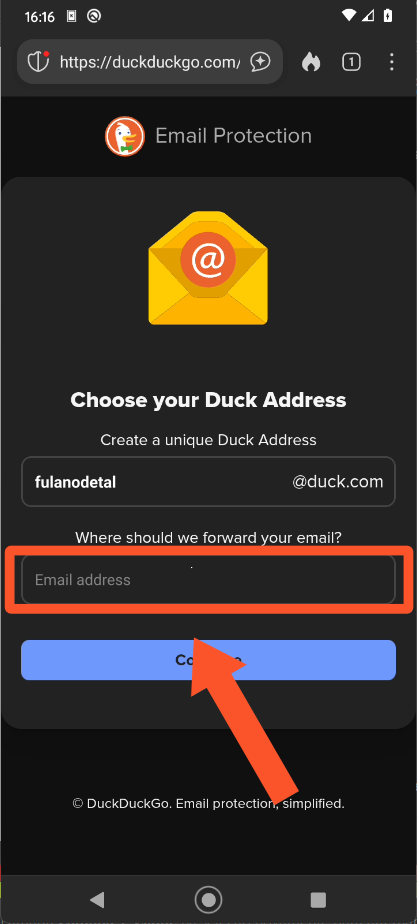
\includegraphics[trim={0cm 0cm 0cm 0cm}, clip, width=\textwidth]{imagens/duckduckgo_10.png}\\[0.2cm]
		\passo{DuckDuckGoOrange}{10}{Seu endereço de e-amil que pretende mascarar}
	\end{minipage}
\end{minipage}

\vspace{0.3cm}
\noindent

% --- BLOCO DE IMAGENS 6 ---
\noindent
\begin{minipage}{\textwidth}
	\centering
	\begin{minipage}{0.45\textwidth}
		\centering
		% Insira o print da tela de criar o endereço @duck.com
		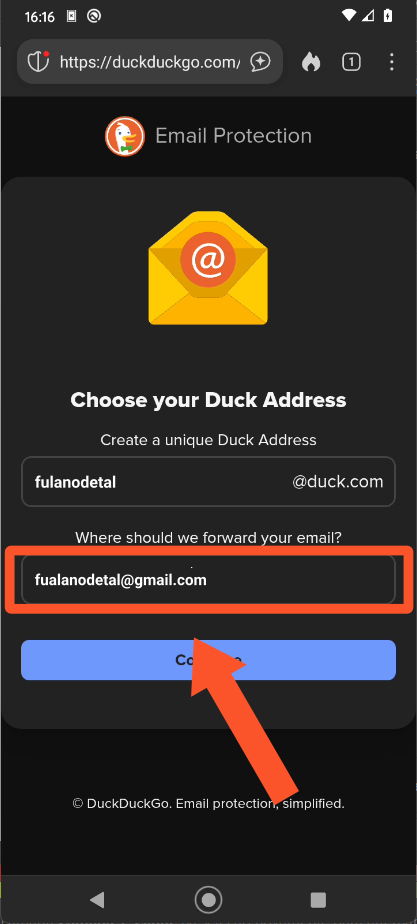
\includegraphics[trim={0cm 0cm 0cm 0cm}, clip, width=\textwidth]{imagens/duckduckgo_11.png}\\[0.2cm]
		\passo{DuckDuckGoOrange}{11}{Exemplo \textbf{CORRETO}}
	\end{minipage}
	\hfill
	\begin{minipage}{0.45\textwidth}
		\centering
		% Insira o print de onde colocar o e-mail verdadeiro
		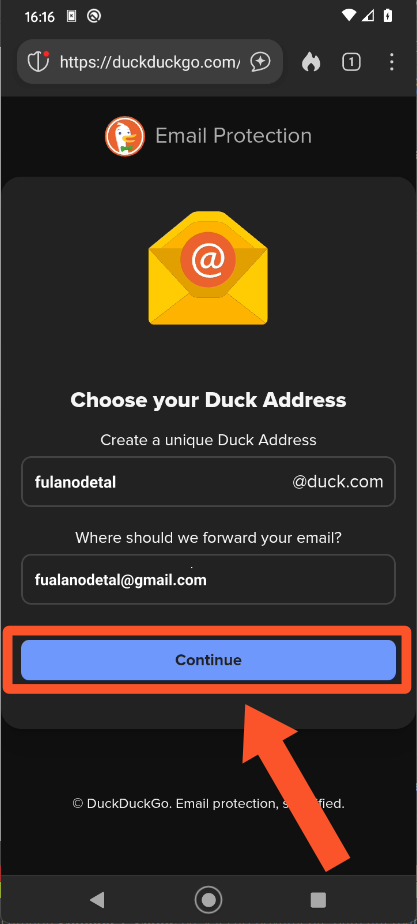
\includegraphics[trim={0cm 0cm 0cm 0cm}, clip, width=\textwidth]{imagens/duckduckgo_12.png}\\[0.2cm]
		\passo{DuckDuckGoOrange}{12}{Toque em \enquote{Continue}}
	\end{minipage}
\end{minipage}

\vspace{0.5cm}
\noindent
Muita atenção, no \textbf{Passo 13} abaixo o Duck vai perguntar se os valores que você digitou nos passo 11 e 9 estão corretos. Se sim, toque no botão azul \enquote{\textbf{This is correct}}. Acompanhe em seguida:

% --- BLOCO DE IMAGENS 7 ---
\noindent
\begin{minipage}{\textwidth}
	\centering
	\begin{minipage}{0.45\textwidth}
		\centering
		% Insira o print da tela de criar o endereço @duck.com
		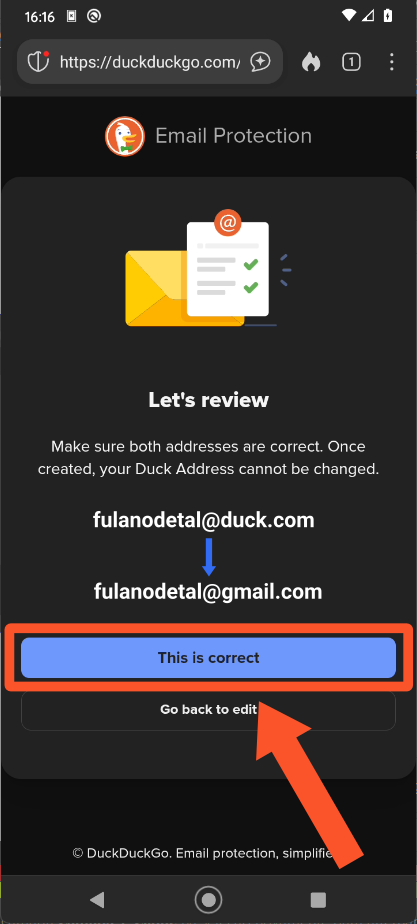
\includegraphics[trim={0cm 0cm 0cm 0cm}, clip, width=\textwidth]{imagens/duckduckgo_13.png}\\[0.2cm]
		\passo{DuckDuckGoOrange}{13}{Toque em \enquote{\textbf{This is correct}} (Está correto)}
	\end{minipage}
	\hfill
	\begin{minipage}{0.45\textwidth}
		\centering
		% Insira o print de onde colocar o e-mail verdadeiro
		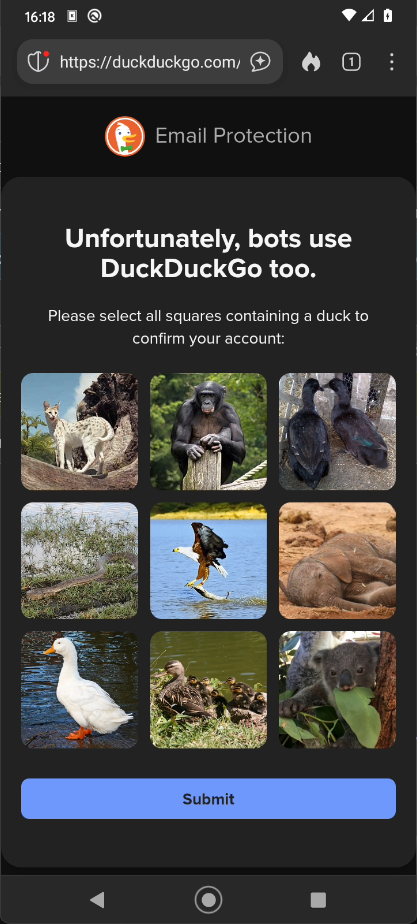
\includegraphics[trim={0cm 0cm 0cm 0cm}, clip, width=\textwidth]{imagens/duckduckgo_14.png}\\[0.2cm]
		\passo{DuckDuckGoOrange}{14}{Marque os patos nas imagens}
	\end{minipage}
\end{minipage}
% --- BLOCO DE IMAGENS 8 ---
\noindent
\begin{minipage}{\textwidth}
	\centering
	\begin{minipage}{0.45\textwidth}
		\centering
		% Insira o print da tela de criar o endereço @duck.com
		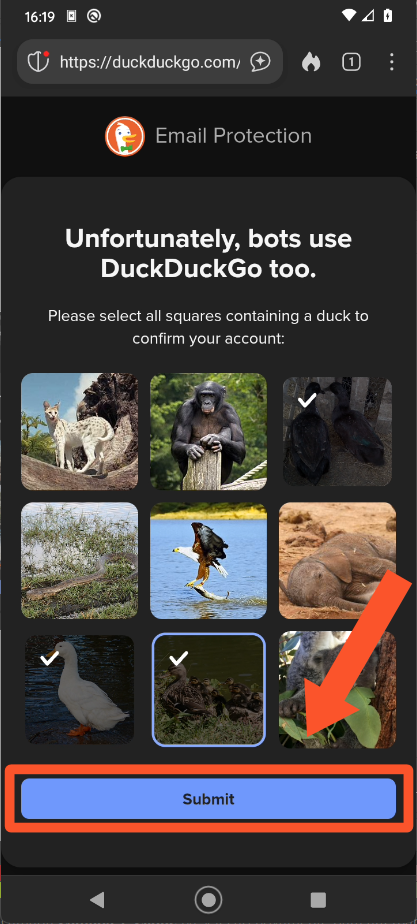
\includegraphics[trim={0cm 0cm 0cm 0cm}, clip, width=\textwidth]{imagens/duckduckgo_15.png}\\[0.2cm]
		\passo{DuckDuckGoOrange}{15}{Toque em \enquote{\textbf{Submit}} (Enviar)}
	\end{minipage}
	\hfill
	\begin{minipage}{0.45\textwidth}
		\centering
		% Insira o print de onde colocar o e-mail verdadeiro
		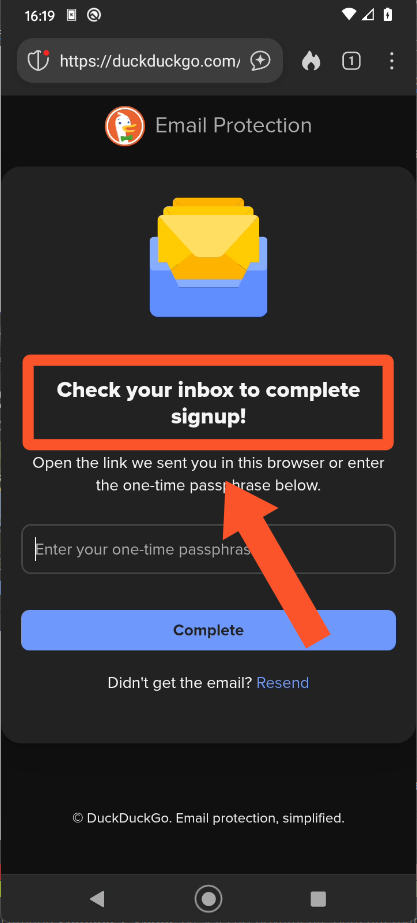
\includegraphics[trim={0cm 0cm 0cm 0cm}, clip, width=\textwidth]{imagens/duckduckgo_16.png}\\[0.2cm]
		\passo{DuckDuckGoOrange}{16}{O Duck enviou uma mensagem para seu e-email}
	\end{minipage}
\end{minipage}

\vspace{0.5cm}
\noindent
\textbf{Passo 16:} O DuckDuckGo enviará uma mensagem de confirmação para o seu e-mail real (aquele que você cadastrou no Passo 11, ex: \textbf{fulanodetal@gmail.com}). 

\vspace{0.3cm}

\begin{tcolorbox}[colback=NordBackground, colframe=red, coltext=white, title=\faExclamationTriangle \ \textbf{Cuidado com a Tradução Automática!}]
	\justifying\noindent
	O e-mail contém uma \textbf{frase de segurança} de 4 palavras (como: \textit{\textbf{thirsty krypton shush audition}}). 
	
	\vspace{0.3cm}
	\noindent
	\textbf{Atenção:} Essa frase \textbf{precisa ser digitada/colada em inglês}. Se o seu Gmail traduzir o e-mail automaticamente para o português, a frase não funcionará. 
	
	\vspace{0.3cm}
	\noindent
	\textbf{Como resolver:} Desative a tradução do navegador ou clique em \enquote{Mostrar original} no Gmail para copiar as palavras exatamente como elas foram enviadas.
\end{tcolorbox}

\vspace{0.3cm}
\noindent
Copie a frase em inglês, cole no campo indicado no aplicativo e clique no botão azul \textbf{\enquote{Complete}} para finalizar o seu escudo de e-mail. Veja no \textbf{Passo 17} abaixo como a mensagem deve ser:
\vspace{0.3cm}

% --- BLOCO DE IMAGENS 9 ---
\noindent
\begin{minipage}{\textwidth}
	\centering
	\begin{minipage}{0.45\textwidth}
		\centering
		% Insira o print da tela de criar o endereço @duck.com
		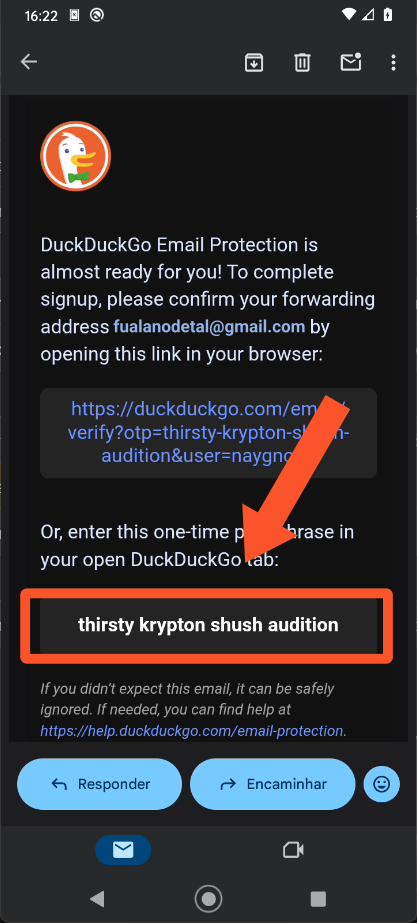
\includegraphics[trim={0cm 0cm 0cm 0cm}, clip, width=\textwidth]{imagens/duckduckgo_17.png}\\[0.2cm]
		\passo{DuckDuckGoOrange}{17}{No seu e-amil, copie a frase senha destacada}
	\end{minipage}
	\hfill
	\begin{minipage}{0.45\textwidth}
		\centering
		% Insira o print de onde colocar o e-mail verdadeiro
		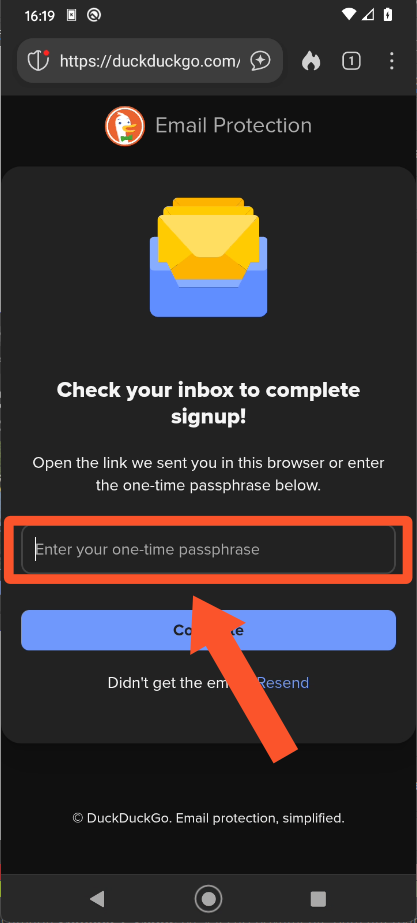
\includegraphics[trim={0cm 0cm 0cm 0cm}, clip, width=\textwidth]{imagens/duckduckgo_18.png}\\[0.2cm]
		\passo{DuckDuckGoOrange}{18}{No navegador DuckdDuckGo, digite/cole no campo destacado}
	\end{minipage}
\end{minipage}

\vspace{0.5cm}
\noindent
\textbf{Atenção:} A imagem do \textbf{Passo 17} acima mostra o conteúdo da mensagem enviada pelo serviço DuckDuckGo para o seu aplicativo de e-mail pessoal. Já a imagem do \textbf{Passo 18} ilustra o retorno à página do navegador para concluir a configuração. É fundamental não confundir o seu \textbf{aplicativo de e-mail} (onde você busca o código) com o \textbf{navegador} (onde você finaliza o cadastro).

% --- BLOCO DE IMAGENS 10 ---
\noindent
\begin{minipage}{\textwidth}
	\centering
	\begin{minipage}{0.45\textwidth}
		\centering
		% Insira o print da tela de criar o endereço @duck.com
		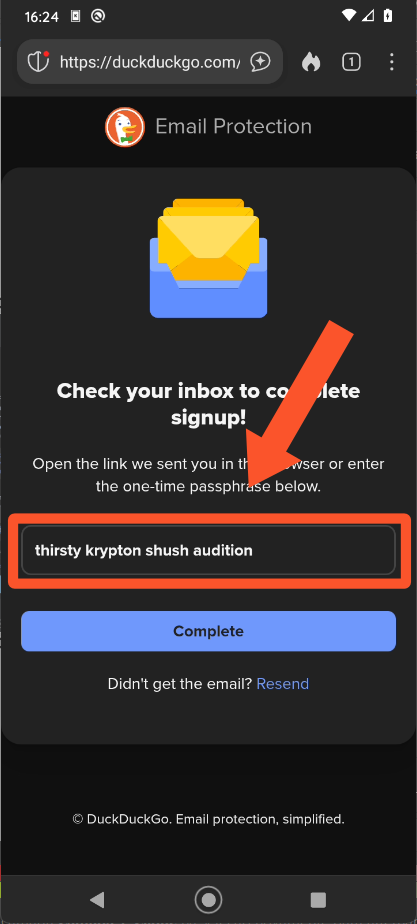
\includegraphics[trim={0cm 0cm 0cm 0cm}, clip, width=\textwidth]{imagens/duckduckgo_19.png}\\[0.2cm]
		\passo{DuckDuckGoOrange}{19}{Forma \textbf{CORRETA} (em inglês)}
	\end{minipage}
	\hfill
	\begin{minipage}{0.45\textwidth}
		\centering
		% Insira o print de onde colocar o e-mail verdadeiro
		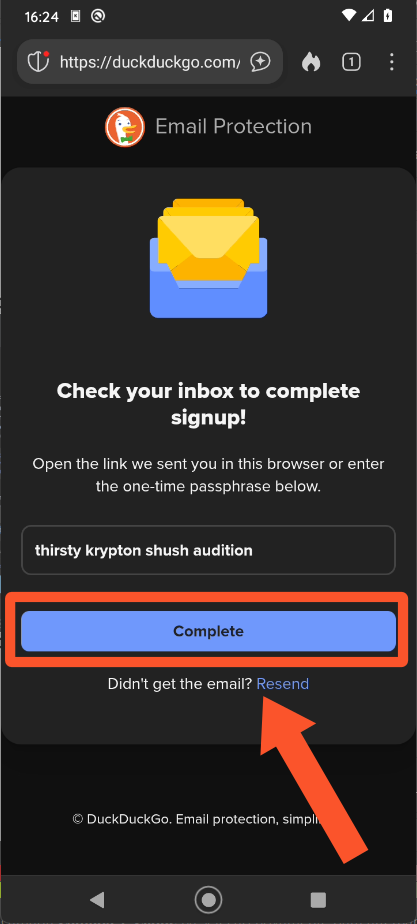
\includegraphics[trim={0cm 0cm 0cm 0cm}, clip, width=\textwidth]{imagens/duckduckgo_20.png}\\[0.2cm]
		\passo{DuckDuckGoOrange}{20}{Toque em \enquote{Complete}}
	\end{minipage}
\end{minipage}

\vspace{0.5cm}

% --- BLOCO DE IMAGENS 11 ---
\noindent
\begin{minipage}{\textwidth}
	\centering
	\begin{minipage}{0.45\textwidth}
		\centering
		% Insira o print da tela de criar o endereço @duck.com
		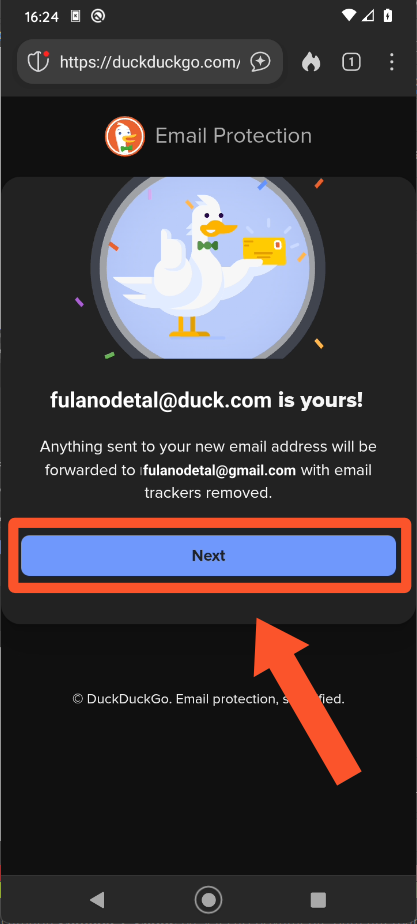
\includegraphics[trim={0cm 0cm 0cm 0cm}, clip, width=\textwidth]{imagens/duckduckgo_21.png}\\[0.2cm]
		\passo{DuckDuckGoOrange}{21}{Toque em \enquote{Next} (Próximo)}
	\end{minipage}
	\hfill
	\begin{minipage}{0.45\textwidth}
		\centering
		% Insira o print de onde colocar o e-mail verdadeiro
		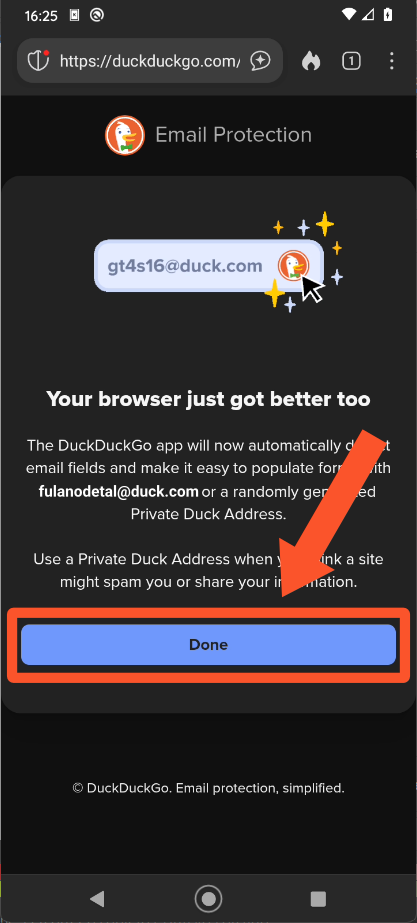
\includegraphics[trim={0cm 0cm 0cm 0cm}, clip, width=\textwidth]{imagens/duckduckgo_22.png}\\[0.2cm]
		\passo{DuckDuckGoOrange}{22}{Toque em \enquote{Done} (Feito)}
	\end{minipage}
\end{minipage}
\vspace{0.5cm}
% --- BLOCO DE IMAGENS 12 ---
\noindent
\begin{minipage}{\textwidth}
	\centering
	\begin{minipage}{0.45\textwidth}
		\centering
		% Insira o print da tela de criar o endereço @duck.com
		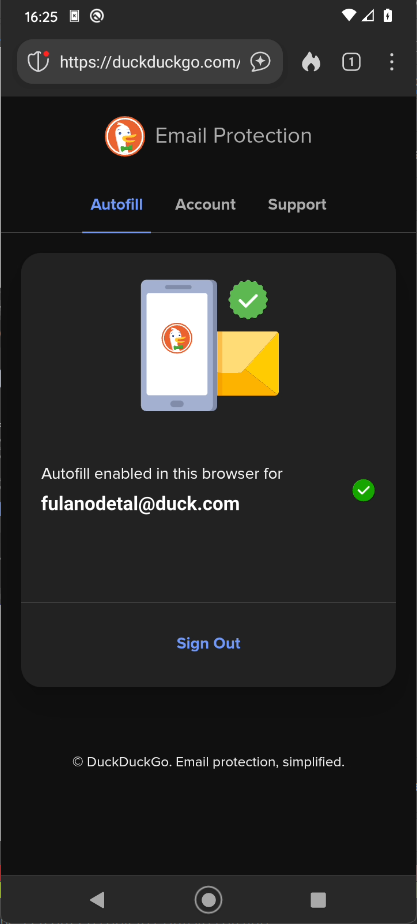
\includegraphics[trim={0cm 0cm 0cm 0cm}, clip, width=\textwidth]{imagens/duckduckgo_23.png}\\[0.2cm]
		\passo{DuckDuckGoOrange}{23}{Cadastro concluído com sucesso!}
	\end{minipage}
	\hfill
	\begin{minipage}{0.45\textwidth}
		\centering
		% Insira o print de onde colocar o e-mail verdadeiro
		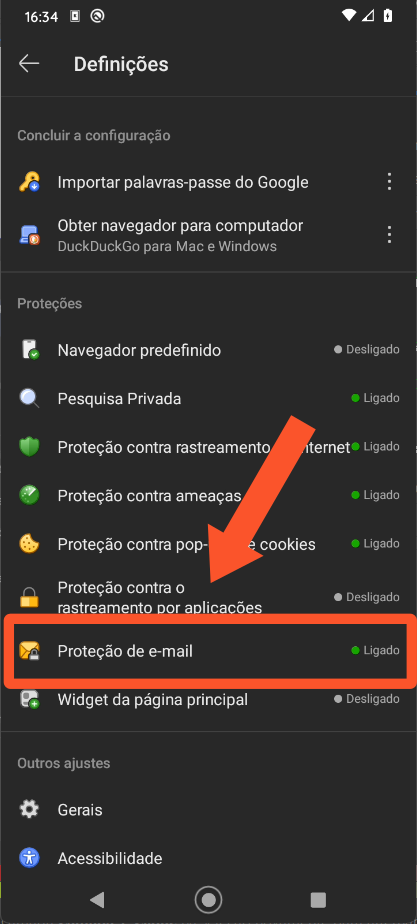
\includegraphics[trim={0cm 0cm 0cm 0cm}, clip, width=\textwidth]{imagens/duckduckgo_24.png}\\[0.2cm]
		\passo{DuckDuckGoOrange}{24}{Verifique se o status está \enquote{Ligado}}
	\end{minipage}
\end{minipage}

\vspace{0.5cm}
\noindent
Para confirmar que a proteção está ativa, acesse as \textbf{Definições} (conforme fizemos no Passo 4) e verifique se o campo \textbf{\enquote{Proteção de e-mail}} está marcado como \textbf{\textcolor{green}{Ligado}}, como demonstrado no \textbf{Passo 24}.


\section*{Usando uma Mascara de E-mail DuckDuckGo}

Acesse qualquer site que exija um e-mail de cadastro utilizando o navegador DuckDuckGo. Note na imagem do \textbf{Passo 25} que o ícone do \enquote{Patinho} aparecerá automaticamente dentro do campo de digitação:

\vspace{0.5cm}

% --- BLOCO DE IMAGENS 13 ---
\noindent
\begin{minipage}{\textwidth}
	\centering
	\begin{minipage}{0.45\textwidth}
		\centering
		% Insira o print da tela de criar o endereço @duck.com
		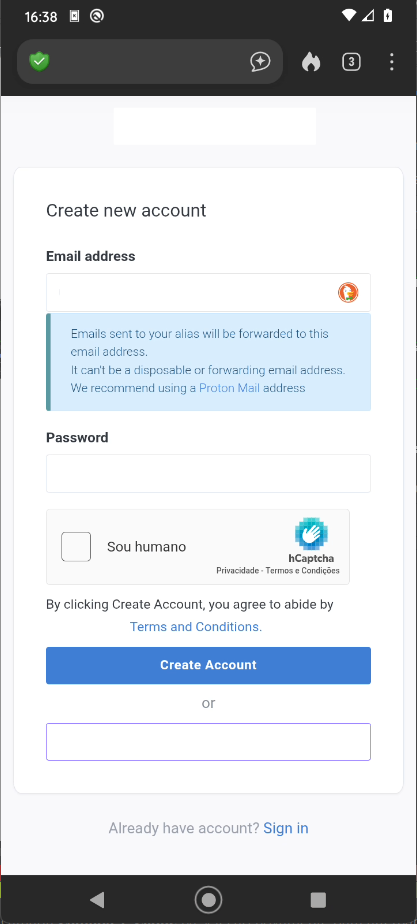
\includegraphics[trim={0cm 0cm 0cm 0cm}, clip, width=\textwidth]{imagens/duckduckgo_25.png}\\[0.2cm]
		\passo{DuckDuckGoOrange}{25}{Identifique o campo de e-mail}
	\end{minipage}
	\hfill
	\begin{minipage}{0.45\textwidth}
		\centering
		% Insira o print de onde colocar o e-mail verdadeiro
		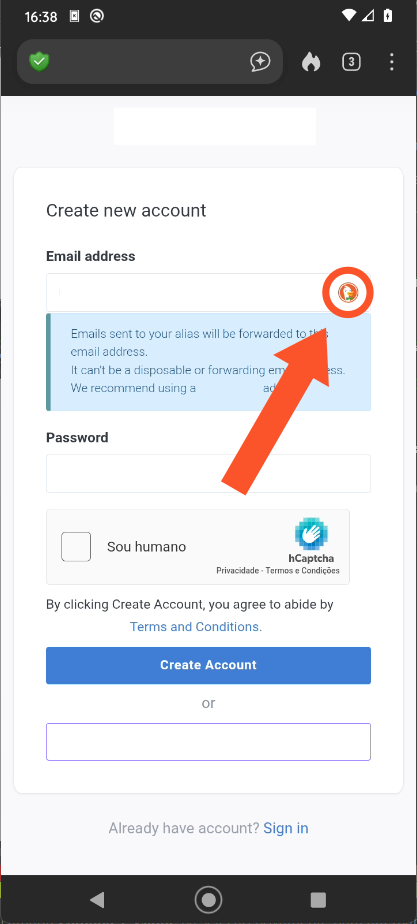
\includegraphics[trim={0cm 0cm 0cm 0cm}, clip, width=\textwidth]{imagens/duckduckgo_26.png}\\[0.2cm]
		\passo{DuckDuckGoOrange}{26}{Toque no ícone do \enquote{Patinho}}
	\end{minipage}
\end{minipage}

\vspace{0.3cm}
\noindent
Ao tocar no ícone, o navegador abrirá um \textbf{painel inferior} com as opções de proteção. Escolha a segunda opção para gerar um endereço totalmente novo, como indica o \textbf{Passo 27}:

% --- BLOCO DE IMAGENS 11 ---
\noindent
\begin{minipage}{\textwidth}
	\centering
	\begin{minipage}{0.45\textwidth}
		\centering
		% Insira o print da tela de criar o endereço @duck.com
		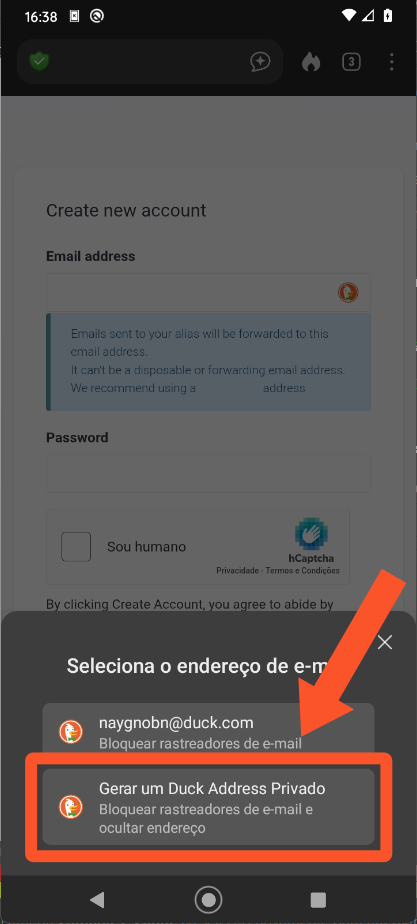
\includegraphics[trim={0cm 0cm 0cm 0cm}, clip, width=\textwidth]{imagens/duckduckgo_27.png}\\[0.2cm]
		\passo{DuckDuckGoOrange}{27}{Toque em \enquote{Gerer um Duck Address Privado}}
	\end{minipage}
	\hfill
	\begin{minipage}{0.45\textwidth}
		\centering
		% Insira o print de onde colocar o e-mail verdadeiro
		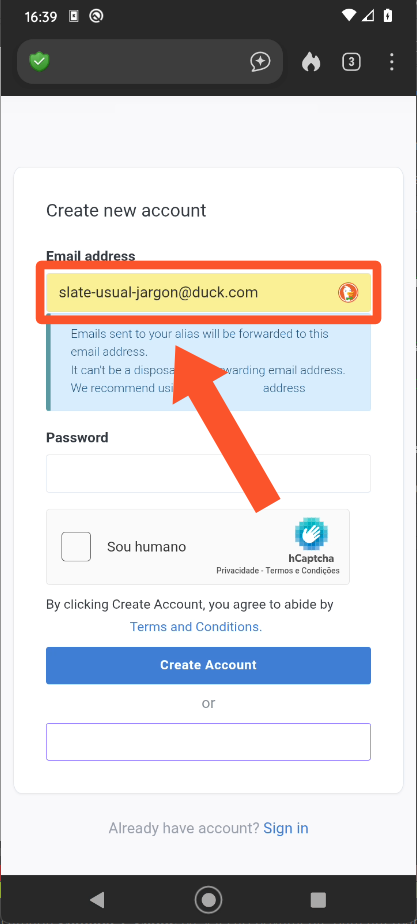
\includegraphics[trim={0cm 0cm 0cm 0cm}, clip, width=\textwidth]{imagens/duckduckgo_28.png}\\[0.2cm]
		\passo{DuckDuckGoOrange}{28}{O campo \textbf{Email address} é preenchido automaticamente}
	\end{minipage}
\end{minipage}

\vspace{0.5cm}
\begin{tcolorbox}[colback=NordBackground, colframe=DuckDuckGoOrange, coltext=white, title=\faMagic \ \textbf{Conforto e Segurança}]
	Pronto! Você se cadastrou no site sem revelar o seu e-mail verdadeiro. A partir de agora, o DuckDuckGo filtrará todos os rastreadores e entregará apenas o conteúdo limpo na sua caixa de entrada oficial.
\end{tcolorbox}

\vspace{0.5cm}
\noindent
\begin{tcolorbox}[colback=NordBackground, colframe=DuckDuckGoOrange, coltext=white, title=\faCheckCircle \ \textbf{Como usar no dia a dia?}]
	Após essa configuração, sempre que você estiver navegando e um site pedir o seu e-mail, o teclado do seu celular (ou o navegador) mostrará o ícone do Patinho. Basta tocar nele e o DuckDuckGo vai gerar um e-mail aleatório (exemplo: \textbf{potato-blue-iron@duck.com}) preenchendo o formulário para você automaticamente!
\end{tcolorbox}

\subsection*{\faEnvelope \ Outra Opção: \textcolor{SimpleLoginDarkPink}{SimpleLogin} (Proton)}
Se você busca uma ferramenta ainda mais robusta, conheça o \textbf{SimpleLogin} \cite{SimpleLogin2026}.

\vspace{0.3cm}
\begin{figure}[h]
	\centering
	
\includegraphics[width=0.4\textwidth]{imagens/simplelogin_dark_logo.png}
	\caption*{(\citeauthor{simplelogin_app} \citefield{simplelogin_app}{version} - Versão oficial)} % Texto manual imitando legenda
\end{figure}

\vspace{0.3cm}
\noindent \justifying %\RaggedRight % Usando RaggedRight para evitar buracos brancos
Ele faz parte do ecossistema da \textit{Proton} e permite criar e gerenciar máscaras de e-mail de forma profissional, inclusive permitindo que você responda e-mails usando a máscara, sem nunca revelar seu endereço real.

\vspace{0.3cm}
\noindent
\begin{center}
	\begin{minipage}{\linewidth}
		\begin{minipage}{0.3\linewidth}
			\centering
			\textbf{\textcolor{BraveOrange}{\faAndroid \ Android}}\\[0.2cm]
			\href{https://bfaxke.short.gy/simplelogin-android}{
				
\includegraphics[width=0.8\linewidth]{imagens/qr_simplelogin_android.png}
			}\\[0.1cm]
			{\scriptsize (Toque ou escaneie)}
		\end{minipage}
		\hfill
		\begin{minipage}{0.3\linewidth}
			\centering
			\textbf{\textcolor{NordText}{\faApple \ iOS / iPhone}}\\[0.2cm]
			\href{https://bfaxke.short.gy/simplelogin-ios}{
				
\includegraphics[width=0.8\linewidth]{imagens/qr_simplelogin_ios.png}
			}\\[0.1cm]
			{\scriptsize (Toque ou escaneie)}
		\end{minipage}
		\hfill
		\begin{minipage}{0.3\linewidth}
			\centering
			\textbf{\textcolor{BitwardenBlue}{\faGlobe \ Web}}\\[0.2cm]
			\href{https://bfaxke.short.gy/simplelogin-email}{
				
\includegraphics[width=0.8\linewidth]{imagens/qr_simplelogin_email.png}
			}\\[0.1cm]
			{\scriptsize (Online)}
		\end{minipage}
		
	\end{minipage}
\end{center}

%\begin{tcolorbox}[colback=NordBackground, colframe=BitwardenBlue, coltext=white, title=\faLightbulb \ \textbf{Outra Opção: SimpleLogin (Proton)}]
%	Se você busca uma ferramenta ainda mais robusta, conheça o \textbf{SimpleLogin} \cite{SimpleLogin2026}.
%	
%	\vspace{0.5cm}
%	\centering
%	
\includegraphics[width=0.4\textwidth]{imagens/simplelogin_dark_logo.png}
%	\caption*{(\citeauthor{simplelogin_app} \citefield{simplelogin_app}{version} - Versão oficial)}
	
%	\vspace{0.5cm}
%	\noindent \justifying
%	Ele faz parte do ecossistema da \textit{Proton} e permite criar e gerenciar máscaras de e-mail de forma profissional, inclusive permitindo que você responda e-mails usando a máscara, sem nunca revelar seu endereço real.
%\end{tcolorbox}

	\newpage
	% 4. REFERÊNCIAS BIBLIOGRÁFICAS
	\printbibliography[heading=bibintoc, title={Referências}]
	\newpage
	\newpage
\thispagestyle{empty}

\vspace*{4cm}

\begin{center}
	\Huge \faCheckCircle \ \textbf{Missão Cumprida!}
	
	\vspace{1cm}
	\Large \justifying \noindent
	A segurança digital não é um destino, mas uma jornada constante. Ao aplicar as dicas deste guia, você deu um passo fundamental para proteger não apenas seus dados, mas o futuro da sua família.
	
	\vspace{2cm}
	
	% --- QR Code para o Repositório ---
	\begin{center}
		\begin{minipage}{0.4\textwidth}
			\centering
			
\includegraphics[width=0.8\linewidth]{imagens/qr_github_guia_seguranca.png}\\
			{\scriptsize \faGithub \ Acompanhe este projeto no GitHub}
		\end{minipage}
	\end{center}
	
	\vfill
	\noindent
	\textit{\enquote{A verdadeira segurança acontece quando o conhecimento se torna um hábito.}}
	
	
	\vspace{1cm}\noindent
	\textbf{Naygno Barbosa Noia} --- 2026
\end{center}
	
\end{document}